% !TEX program = xelatex
% Base acadêmica da UnDF para o Projeto Final — Empresa Júnior
% Conteúdo-fonte: ../projeto-empresa-junior.md
\documentclass[
  12pt,
  openright,
  oneside,
  a4paper,
  brazilian
]{abntex2}

% -----------------------------------------------------------------------------
% Pacotes
% -----------------------------------------------------------------------------
\usepackage{fontspec}
\defaultfontfeatures{Ligatures=TeX}
\setmainfont{Times New Roman}
\setsansfont{Times New Roman}
\usepackage{microtype}
\usepackage{indentfirst}
\usepackage{graphicx}
\usepackage{booktabs}
\usepackage{tabularx}
\usepackage{longtable}
\usepackage{array}
\usepackage{enumitem}
\usepackage{xcolor}
\usepackage{url}
\usepackage{hyperref}
\usepackage{csquotes}
\usepackage[
  backend=biber,
  style=abnt,
  sccite=false,
  accite=false,
  ittitles=true,
  giveninits=true,
  uniquename=false,
  maxcitenames=3,
  maxbibnames=99
]{biblatex}
\addbibresource{referencias.bib}
\graphicspath{{figuras/}}
\usepackage{pgfgantt}
\usepackage[framemethod=tikz]{mdframed}
\usepackage{tikz}
\usetikzlibrary{arrows.meta, positioning, calc}

\usepackage{listings}
\usepackage{xcolor}

\colorlet{punct}{red!60!black}
\colorlet{delim}{blue!60!black}
\colorlet{numb}{magenta!60!black}

\lstdefinelanguage{json}{
    basicstyle=\small\ttfamily,
    numbers=left,
    numberstyle=\tiny\color{gray},
    stepnumber=1,
    numbersep=8pt,
    showstringspaces=false,
    breaklines=true,
    frame=lines,
    backgroundcolor=\color{gray!5},
    literate=
     *{0}{{{\color{numb}0}}}{1}
      {1}{{{\color{numb}1}}}{1}
      {2}{{{\color{numb}2}}}{1}
      {3}{{{\color{numb}3}}}{1}
      {4}{{{\color{numb}4}}}{1}
      {5}{{{\color{numb}5}}}{1}
      {6}{{{\color{numb}6}}}{1}
      {7}{{{\color{numb}7}}}{1}
      {8}{{{\color{numb}8}}}{1}
      {9}{{{\color{numb}9}}}{1}
      {:}{{{\color{punct}{:}}}}{1}
      {,}{{{\color{punct}{,}}}}{1}
      {\{}{{{\color{delim}{\{}}}}{1}
      {\}}{{{\color{delim}{\}}}}}{1}
      {[}{{{\color{delim}{[}}}}{1}
      {]}{{{\color{delim}{]}}}}{1},
}

% -----------------------------------------------------------------------------
% Dados do trabalho
% -----------------------------------------------------------------------------
\newcommand{\instituicaoNome}{Universidade do Distrito Federal Professor Jorge Amaury Maia Nunes}
\newcommand{\instituicaoSigla}{UnDF}
\newcommand{\professorNome}{Prof. Rodrigo Torres Carrilho da Costa}
\newcommand{\cidadeNome}{Brasília}
\newcommand{\anoEntrega}{jul. 2026}
\newcommand{\disciplina}{Estágio Empresarial II}
\newcommand{\bcb}{Banco Central do Brasil}
\newcommand{\sfn}{Sistema Financeiro Nacional}

\titulo{Jataí: empresa júnior para formação técnica em
\newline\texorpdfstring{\textit{Open Finance}}{Open Finance}}
\autor{Karoline Rodrigues Costa \\ Leonardo Brito Gomes \\ Luiz Gustavo Silva Carvalho}
\local{\cidadeNome}
\data{\anoEntrega}
\instituicao{%
  \instituicaoNome{} (\instituicaoSigla)
}
\tipotrabalho{Trabalho acadêmico}
\preambulo{Trabalho acadêmico apresentado à \instituicaoNome{} (\instituicaoSigla), como entrega final para a Unidade Curricular de \disciplina, sob orientação do \professorNome.}

% -----------------------------------------------------------------------------
% Aparência e formatação
% -----------------------------------------------------------------------------
\definecolor{jatai}{HTML}{B56B1C}
\definecolor{linkcolor}{HTML}{5B3510}

\hypersetup{
  pdftitle={Jataí: proposta de empresa júnior para formação técnica em Open Finance},
  pdfauthor={Karoline Rodrigues Costa; Leonardo Brito Gomes; Luiz Gustavo Silva Carvalho},
  pdfsubject={Projeto acadêmico de empresa júnior},
  hidelinks,
  bookmarksdepth=4
}

\setlength{\parindent}{1.25cm}
\setlength{\parskip}{0pt}
\setlist[itemize]{noitemsep,topsep=0.5em}
\setlist[enumerate]{noitemsep,topsep=0.5em}
\renewcommand{\arraystretch}{1.25}
\urlstyle{same}

% Referências em espaço simples, separadas entre si por uma linha simples.
\AtBeginBibliography{%
  \SingleSpacing
  \setlength{\bibitemsep}{\baselineskip}
}

\newcolumntype{Y}{>{\raggedright\arraybackslash}X}
\newcommand{\openfinance}{\textit{Open Finance}}
\newcommand{\opensource}{\textit{open source}}
\newcommand{\sandbox}{\textit{sandbox}}

\renewcommand{\ABNTEXchapterfont}{\rmfamily}
\renewcommand{\ABNTEXsectionfont}{\rmfamily}
\renewcommand{\ABNTEXsubsectionfont}{\rmfamily}

\makepagestyle{academico}
\makeevenhead{academico}{}{}{\ABNTEXfontereduzida\thepage}
\makeoddhead{academico}{}{}{\ABNTEXfontereduzida\thepage}
\makeevenfoot{academico}{}{}{}
\makeoddfoot{academico}{}{}{}

\begin{document}
\selectlanguage{brazilian}
\frenchspacing

% -----------------------------------------------------------------------------
% Elementos pré-textuais
% -----------------------------------------------------------------------------
\pretextual

\begin{capa}
  \centering
  
\includegraphics[width=5cm]{undf-marca-vertical.png}\\[0.8cm]

  \vfill
  {\ABNTEXchapterfont\large\imprimirautor}

  \vfill
  {\ABNTEXchapterfont\bfseries\Large\imprimirtitulo}

  \vfill
  \imprimirlocal\\
  \imprimirdata
\end{capa}

\begin{folhaderosto}
  \centering
  {\ABNTEXchapterfont\large\imprimirautor}

  \vfill
  {\ABNTEXchapterfont\bfseries\Large\imprimirtitulo}

  \vfill
  \hspace*{\fill}
  \begin{minipage}{0.52\textwidth}
    \SingleSpacing
    \imprimirpreambulo
  \end{minipage}

  \vfill
  \imprimirlocal\\
  \imprimirdata
\end{folhaderosto}

\pdfbookmark[0]{\contentsname}{toc}
\tableofcontents*
\cleardoublepage

% -----------------------------------------------------------------------------
% Elementos textuais
% -----------------------------------------------------------------------------
\textual
\pagestyle{academico}
\aliaspagestyle{chapter}{academico}

\chapter{Introdução}

% Escreva aqui a introdução.

% Descrever a dor do cliente e referenciar a existência do Open Finance

% https://openfinancebrasil.org.br/2021/05/18/open-banking-no-mundo-2/
% https://openfinancebrasil.org.br/2021/05/18/evolucao-regulatoria-do-open-finance-no-brasil/

O \bcb{} observava a tendência mundial de integração financeira entre dados e usuários, com o objetivo de quebrar as fronteiras entre instituições financeiras por meio da integração de seus respectivos sistemas. Esse fenômeno foi observado principalmente no Reino Unido, em 2018 \parencite{openfinancebrasil2021mundo}. A iniciativa do Open Finance foi criada como resultado da colaboração do \bcb{} com mercado, reguladores e outras partes interessadas.

\begin{citacao}
Essa iniciativa tem como objetivo aumentar a eficiência no mercado de crédito e de pagamentos no Brasil, mediante a promoção de ambiente de negócio mais inclusivo e competitivo, preservando a segurança do sistema financeiro e a proteção dos consumidores.

\parencite{bcb2019comunicado33455}
\end{citacao}

Mais de cinco anos após a sua criação, o Open Finance brasileiro segue sendo o maior mundialmente. Segundo o \bcb{} \citeyear{bcbOpenFinanceEntender}, mais de 116 bilhões de brasileiros autorizaram o compartilhamento de seus dados financeiros via Open Finance.

Nesse sentido, é de extrema importância a existência de material de apoio para o aprendizado e formação técnica de novos profissionais que planejam desenvolver soluções de integração financeira dentro do \sfn{}. Nesse princípio fundamenta-se a Jataí, pois os materiais disponibilizados atualmente pelo \bcb{} e pela Área do Desenvolvedor do Open Finance Brasil, relativos ao Open Finance e à integração de sistemas financeiros como um todo, são suficientes para demonstrar a existência de uma base técnica padronizada, com especificações de APIs, requisitos não funcionais, limites de tráfego, informações de desempenho e orientações de implementação \parencite{openfinancebrasilAreaDesenvolvedor}, focando principalmente em instituições parceiras (bancos e fintechs), mas não suprem a necessidade de um nicho específico de novos desenvolvedores que aspiram aprender mais sobre o funcionamento de sistemas bancários.

\section{Objetivo geral}

% Escreva aqui o objetivo geral.

A Jataí tem como objetivo democratizar o acesso ao estudo de APIs financeiras e integrações por meio do Open Finance dentro do ambiente universitário, por meio de uma abordagem simplificada, abstraindo a complexidade técnica e regulatória atrelada à sistemas bancários, levando em consideração o que se faz realmente relevante na formação profissional do estudante. 

\section{Objetivos específicos}

\begin{itemize}
  \item Desenvolver materiais didáticos introdutórios sobre APIs financeiras, Open Finance, autenticação, segurança e integração entre sistemas, com linguagem acessível ao público universitário.

  \item Estruturar uma trilha de aprendizagem progressiva que conduza o estudante dos conceitos básicos de consumo de APIs até a compreensão de fluxos mais complexos, como OAuth2, OpenID Connect, webhooks, Pix, dados sintéticos e testes de integração.

  \item Criar e manter um ambiente de \textit{sandbox} educacional para simulação de APIs financeiras, permitindo que estudantes, desenvolvedores autônomos e pequenas startups validem protótipos sem depender de dados bancários reais ou de integrações com sistemas de produção.

  \item Disponibilizar ferramentas práticas de apoio ao desenvolvimento, como API bancária simulada, ambiente de iniciação de pagamentos, servidor de autorização, telemetria de requisições e gerador de dados financeiros sintéticos.

  \item Reduzir as barreiras técnicas, financeiras e regulatórias enfrentadas por iniciantes no estudo de sistemas financeiros digitais, oferecendo acesso gratuito ou de baixo custo a ambientes de teste, documentação e exemplos práticos.

  \item Aproximar universidade, estudantes, comunidades de tecnologia, bancos e fintechs por meio de oficinas, desafios técnicos, hackathons, documentação aberta e projetos orientados à formação profissional.
\end{itemize}

\section{Metodologia}

% Escreva aqui a metodologia.

A seção de metodologia será responsável por apresentar o caminho lógico que resultou na criação da Jataí. Serão apresentadas as etapas de pesquisa exploratória, que será utilizada para mapear o Open Finance, compreender os problemas enfrentados por estudantes e desenvolvedores iniciantes e orientar a formulação da Jataí; de pesquisa documental, responsável por fundamentar, por meio de documentos legais e técnicos, a constituição da empresa júnior; de levantamento de requisitos, que busca definir o que a empresa deve possuir para agregar valor diante do problema apresentado; de prototipagem, que apresenta um conjunto de protótipos desenvolvidos com base nos requisitos levantados; e de plano de validação com os usuários, que busca traçar uma estratégia para como devemos verificar se a entrega de valor está de acordo com as expectativas do público-alvo.

% pesquisa exploratoria

A pesquisa exploratória parte do reconhecimento de que o Open Finance constitui um sistema de integração financeira complexo, voltado à padronização do compartilhamento de dados e serviços no âmbito do \sfn{} brasileiro. Embora existam materiais oficiais disponibilizados publicamente, esses documentos apresentam caráter predominantemente técnico e normativo, sendo direcionados principalmente a instituições participantes e desenvolvedores envolvidos na implementação de soluções financeiras. Nesse contexto, identifica-se uma lacuna educacional para estudantes e desenvolvedores iniciantes, que necessitam não apenas compreender os fundamentos teóricos do ecossistema, mas também praticar sua aplicação em ambientes simulados, acessíveis e pedagogicamente orientados. É a partir dessa lacuna que se fundamenta a proposta da Jataí.

% pesquisa documental

A pesquisa documental busca organizar a base jurídica, regulatória e técnica que fundamenta a Jataí como empresa júnior voltada à educação em tecnologias de integração financeira. Essa etapa considera documentos legais relacionados à constituição de empresas juniores, materiais oficiais do Banco Central do Brasil e referências técnicas do Open Finance Brasil, a fim de delimitar a atuação da empresa como iniciativa educacional, sem operação financeira real, sem tratamento de dados bancários reais e sem integração com ambientes de produção.

No aspecto jurídico, a pesquisa documental se apoia na Lei nº 13.267/2016, que disciplina a criação e a organização das empresas juniores, estabelecendo sua natureza educacional, sua vinculação a instituições de ensino superior e a vedação de distribuição de resultados financeiros entre seus integrantes. Também são considerados dispositivos gerais do Código Civil relativos às associações civis, uma vez que a empresa júnior assume essa forma jurídica.

No aspecto regulatório, a análise considera documentos do Banco Central do Brasil relacionados ao Open Finance e ao Sistema Financeiro Aberto, com o objetivo de compreender os limites da atuação da Jataí. Como a proposta se restringe à simulação, ao uso de dados sintéticos, à documentação técnica e à prototipagem educacional, a empresa não se caracteriza como instituição financeira, instituição de pagamento ou participante regulado do Open Finance.

No aspecto técnico, a pesquisa documental contempla materiais da Área do Desenvolvedor do Open Finance Brasil, que reúnem especificações de APIs, requisitos não funcionais, limites de tráfego, padrões de implementação e orientações voltadas às instituições participantes. Esses documentos servem como referência para a definição dos conteúdos e funcionalidades simuladas pela Jataí, sem que isso implique integração com sistemas reais de produção.

% levantamento de requisitos

No levantamento de requisitos, busca-se delimitar o escopo da Jataí, através de requisitos funcionais e não funcionais, definindo os elementos essenciais que seus produtos devem apresentar para responder à dor do cliente. Essa etapa permite estabelecer quais funcionalidades, conteúdos e critérios mínimos são necessários para que as soluções propostas agreguem valor ao público-alvo.

Dentro disso, podemos definir alguns requisitos funcionais:

\begin{itemize}
  \item Permitir que o usuário consuma uma API bancária simulada para consulta de dados financeiros fictícios.

  \item Disponibilizar um ambiente de \textit{sandbox} para testes de integração com APIs financeiras.

  \item Simular fluxos de autenticação e autorização utilizados em integrações financeiras.

  \item Gerar dados financeiros sintéticos para uso em testes, protótipos e atividades educacionais.

  \item Disponibilizar documentação técnica e exemplos práticos para apoiar o aprendizado dos usuários.

  \item Registrar informações básicas sobre requisições, respostas e erros para fins de estudo, depuração e telemetria.
\end{itemize}

Também são definidos requisitos não funcionais, responsáveis por estabelecer critérios de qualidade, restrições e condições de funcionamento da plataforma:

\begin{itemize}
  \item Utilizar apenas dados sintéticos, sem tratamento de dados bancários reais.

  \item Apresentar documentação clara, progressiva e acessível para estudantes e desenvolvedores iniciantes.

  \item Manter limites de uso compatíveis com a infraestrutura disponível.

  \item Garantir segurança básica nas comunicações e nos fluxos simulados de autenticação.

  \item Preservar estabilidade suficiente para uso em oficinas, aulas, hackathons e testes acadêmicos.

  \item Permitir evolução modular dos produtos conforme novas necessidades educacionais e técnicas forem identificadas.
\end{itemize}

% prototipagem



% plano de validação

Para validar se o que foi produzido realmente está alinhado com o que o público-alvo está buscando, a Jataí planeja apresentar seus protótipos em contextos educacionais e de inovação, combinando oficinas, demonstrações guiadas e coleta estruturada de feedback. Eventos como a Campus Party representam uma alternativa relevante para essa etapa, pois contam com programas voltados à exposição de projetos estudantis, troca de experiências, networking e validação de ideias, como o Campus Future \parencite{campuspartyCampusFuture}, além de iniciativas voltadas a startups, mentorias, conexão com mercado e possibilidades de parcerias estratégicas, como o Campus Startups \parencite{campuspartyCampusStartups}. Nesse sentido, a validação da Jataí poderá ocorrer em hackathons, comunidades online de desenvolvimento, semanas acadêmicas, laboratórios universitários e eventos de tecnologia.

Além desses espaços, a Jataí poderá buscar parcerias com instituições financeiras, fintechs, cooperativas de crédito e empresas de tecnologia interessadas em apoiar a formação de novos talentos. Essas parcerias deverão ter caráter educacional, sem acesso a dados bancários reais e sem integração com ambientes de produção, podendo envolver mentorias técnicas, desafios práticos, avaliação dos protótipos, palestras, apoio a oficinas e validação de casos de uso simulados. Também poderão ser realizadas turmas piloto com estudantes da UnDF e de outras instituições de ensino, permitindo avaliar critérios como clareza da documentação, facilidade de consumo das APIs simuladas, compreensão dos fluxos de autenticação, estabilidade do \textit{sandbox} e percepção de valor pelos usuários.

\chapter{Identificação da Empresa}
\label{cap:identificacao_empresa}

\section{Dados cadastrais}
\label{sec:dados_cadastrais}

\begin{description}
  \item[Nome:] Jataí.
  \item[Slogan:] \textit{"Democratizando a engenharia de software para o Open Finance."}
  \item[Ramo de atuação:] Tecnologia da Informação, com foco no ecossistema de Open Finance e no desenvolvimento de ferramentas de infraestrutura lógica para simulação de sistemas financeiros, como APIs bancárias simuladas, ambientes de \textit{sandbox}, servidores de autorização, ferramentas de telemetria e geradores de dados financeiros sintéticos.
  \item[Natureza jurídica:] Associação Civil de Direito Privado, sem fins lucrativos, estruturada como Empresa Júnior nos termos da Lei Federal nº 13.267/2016 \cite{brasil2016empresa}. A Jataí possui finalidade educacional e e vinculação acadêmica à \instituicaoNome{} (\instituicaoSigla), sendo vedada a distribuição de lucros ou excedentes financeiros entre seus integrantes. Toda eventual receita obtida será reinvestida na manutenção da plataforma, na infraestrutura tecnológica, na capacitação dos membros e no desenvolvimento das atividades-fim da empresa.
  \item[Descrição:] A Jataí é uma empresa júnior voltada à democratização do acesso a ambientes de teste e aprendizagem em APIs financeiras. Sua proposta consiste em oferecer soluções tecnológicas acessíveis para estudantes, desenvolvedores iniciantes, desenvolvedores autônomos e pequenas startups que desejam compreender, construir protótipos e validar integrações inspiradas no Open Finance sem depender de dados bancários reais ou de acesso a sistemas financeiros de produção. A Jataí busca aproximar o público universitário das práticas utilizadas no mercado financeiro digital.
\end{description}

\section{Logomarca e identidade visual}
\label{sec:logomarca}

A identidade visual da Jataí busca harmonizar a precisão da engenharia de \textit{software} com a simbologia de colaboração e construção em rede inerente ao ecossistema de \openfinance{}. A Figura~\ref{fig:logo_jatai} apresenta a logomarca oficial da empresa.

\begin{figure}[htbp]
    \centering
    
\includegraphics[width=0.45\textwidth]{logo_jatai.png}
    \caption{Logomarca Oficial da Jataí.}
    \label{fig:logo_jatai}
    \legend{Fonte: Elaborado pelos autores (2026).}
\end{figure}

\subsection{Conceituação semiótica do design}
O design da marca pauta-se tanto em uma tipografia característica quanto no hexágono como pingo do "I". O qual remete à estrutura dos favos de mel produzidos pela abelha Tetragonisca angustula (Jataí), símbolo nacional de organização e trabalho coletivo, bem como representa a modularidade computacional, a arquitetura de dados e os blocos de integração (\textit{building blocks}) característicos das APIs de \openfinance{}.

\section{Descrição geral da empresa}
\label{sec:descricao_empresa}

A Jataí é uma empresa júnior voltada à democratização do acesso a ambientes de teste, simulação e aprendizagem prática em APIs financeiras. Sua proposta consiste em oferecer soluções tecnológicas acessíveis e de alta fidelidade técnica para estudantes, desenvolvedores iniciantes, pesquisadores e \textit{fintechs} em fase inicial.

Por meio do fornecimento de \textit{sandboxes} simulados, servidores de autorização FAPI, geradores de dados sintéticos e injetores de caos, a Jataí permite que seus usuários compreendam, construam protótipos e validem integrações inspiradas no \openfinance{} sem depender de dados bancários reais ou de credenciais de produção de instituições financeiras, reduzindo significativamente as barreiras de entrada no setor.

\section{Missão, visão e valores}
\label{sec:missao_visao_valores}

\subsection{Missão}
Promover a formação técnica de estudantes, desenvolvedores e pesquisadores por meio da oferta de ambientes de simulação, ferramentas computacionais e materiais educacionais voltados ao ecossistema do \openfinance{}, contribuindo para reduzir as barreiras de entrada existentes no desenvolvimento de soluções financeiras digitais e aproximando o meio acadêmico das tecnologias empregadas pelo mercado.

\subsection{Visão}
Consolidar-se como referência nacional entre as empresas juniores na produção de ferramentas educacionais voltadas ao \openfinance{}, sendo reconhecida pela qualidade técnica de suas soluções, pelo incentivo à inovação aberta e pela contribuição para a formação de profissionais capacitados a atuar no desenvolvimento de sistemas financeiros digitais.

\subsection{Valores}
Os princípios que orientam a atuação da Jataí refletem tanto sua natureza acadêmica quanto seu compromisso com a disseminação do conhecimento e o desenvolvimento responsável de tecnologias:
\begin{itemize}
    \item{Democratização do acesso:} disseminação irrestrita do conhecimento e de ferramentas de integração financeira;
    \item{Ética e transparência:} atuação responsável no desenvolvimento de soluções computacionais e na gestão da empresa júnior;
    \item{Padrões abertos e interoperabilidade:} adoção rigorosa de boas práticas de engenharia de \textit{software} e especificações abertas;
    \item{Cultura \textit{Open Source}:} valorização da colaboração, do compartilhamento de código e do aprendizado em comunidade;
    \item{Inovação e experimentação segura:} incentivo ao aprendizado prático e à tolerância a falhas em ambientes simulados;
    \item{Segurança e privacidade:} respeito rigoroso às normas de segurança da informação e proteção de dados (\textit{Privacy by Design}).
\end{itemize}

\section{História da criação}
\label{sec:historia_criacao}

A criação da Jataí fundamenta-se na identificação de uma lacuna existente entre a ampla disponibilidade de especificações técnicas do ecossistema de \openfinance{} e a dificuldade enfrentada por estudantes e desenvolvedores iniciantes para transformar esse conhecimento em experiência prática. Embora o \bcb{} e a estrutura de governança do Open Finance Brasil disponibilizem documentação abrangente sobre padrões de integração, autenticação, requisitos de segurança e funcionamento das APIs, esses materiais são direcionados principalmente às instituições participantes e aos profissionais já inseridos no mercado, exigindo conhecimentos prévios de arquitetura de software, protocolos de segurança e infraestrutura computacional.

Paralelamente, observou-se que os ambientes de testes disponibilizados por instituições financeiras possuem finalidade distinta daquela necessária ao contexto educacional. Em geral, esses ambientes são concebidos para validar integrações específicas com seus próprios serviços, reproduzindo requisitos técnicos e regulatórios compatíveis com aplicações reais, mas sem priorizar aspectos didáticos, simplicidade de implantação ou flexibilidade para experimentação por estudantes.

Diante desse cenário, concebeu-se a Jataí como uma empresa júnior dedicada ao desenvolvimento de uma infraestrutura educacional voltada ao aprendizado de tecnologias empregadas no ecossistema financeiro digital. Sua proposta consiste em disponibilizar um conjunto integrado de ferramentas, documentação e ambientes de simulação capazes de reduzir a complexidade inicial enfrentada por novos desenvolvedores, permitindo que conceitos relacionados a APIs financeiras, autenticação, dados sintéticos e integração entre sistemas sejam explorados de forma segura, acessível e alinhada às práticas adotadas pelo mercado.

Assim, a Jataí busca atuar como elemento de aproximação entre universidade e setor produtivo, oferecendo aos estudantes oportunidades de aprendizado prático e contribuindo para a formação de profissionais preparados para os desafios tecnológicos do \sfn{}.

\chapter{Problema da comunidade}
\label{cap:problema_comunidade}
O avanço e a consolidação do ecossistema de \openfinance{} no Brasil, impulsionados pela regulamentação do \bcb{}, desencadearam uma profunda transformação no setor financeiro, exigindo profissionais com domínio prático em arquitetura de APIs, autenticação via OpenID Connect/FAPI, criptografia e sistemas de alta disponibilidade. Contudo, identifica-se uma contradição no mercado, ao passo que a demanda por desenvolvedores qualificados cresce o acesso à infraestrutura prática de aprendizado permanece restrito. 

Os ambientes de testes (\sandbox{}) mantidos pelas grandes instituições bancárias e \textit{fintechs} consolidadas não foram concebidos com finalidade didática. Como consequência, os estudantes e desenvolvedores são forçados a limitar sua formação à teoria ou a utilizar simuladores genéricos desatualizados que não reproduzem a arquitetura real do \sfn{}.

\section{Metodologia de identificação do problema}
\label{sec:metodologia_identificacao}

A constatação e o mapeamento desta necessidade fundamentaram-se em três pilares metodológicos de investigação:

\begin{enumerate}
    \item{Análise de comportamento em comunidades de desenvolvedores:} mapeamento de tópicos recorrentes e dúvidas frequentes, onde programadores iniciantes relatam recorrentemente a impossibilidade de testar chamadas FAPI sem credenciais institucionais;
    \item{Benchmarking de ambientes \textit{Sandbox} existentes:} estudo comparativo das plataformas de testes disponibilizadas pelos principais conglomerados bancários nacionais, constatando a ausência de recursos didáticos, como geradores automatizados de dados sintéticos ou simuladores de injeção de falhas para testes de resiliência.
\end{enumerate}

\section{Caracterização do público-alvo}
\label{sec:publico_alvo}

O público impactado e atendido pelas soluções da Jataí divide-se em três segmentos bem delimitados, apresentados na Tabela~\ref{tab:publico_alvo}.

\begin{table}[htbp]
\centering
\caption{Segmentação e necessidades do público-alvo.}
\label{tab:publico_alvo}
\begin{tabular}{|p{4.5cm}|p{5cm}|p{5cm}|}
\hline
\textbf{Grupo do Público-Alvo} & \textbf{Perfil do Usuário} & \textbf{Principal Necessidade} \\ \hline
\textbf{Estudantes e Pesquisadores} & Alunos de graduação, pós-graduação e docentes de TI. & Acesso gratuito e simplificado a \textit{sandboxes} locais para TCCs e disciplinas práticas. \\ \hline
\textbf{Desenvolvedores Autônomos / Iniciantes} & Programadores em transição de carreira ou criando portfólio. & Documentação clara, execução sem custo via Docker e baixo tempo para a primeira requisição. \\ \hline
\textbf{Startups / Early-Stage \textit{Fintechs}} & Pequenas equipes de produto em fase de ideação/validação. & Validação rápida de protótipos e testes de carga/falhas sem depender de contratos bancários. \\ \hline
\end{tabular}
\legend{Fonte: Elaborado pelos autores (2026).}
\end{table}

\section{Impacto do problema na comunidade}
\label{sec:impacto_problema}

A persistência dessas barreiras tecnológicas gera impactos negativos em três dimensões principais:

\subsection{Impacto educacional}
Aprofunda o descompasso entre o ensino universitário tradicional e as exigências do mercado de trabalho financeiro. Os graduandos ingressam no mercado de trabalho sem vivência prática em protocolos modernos de segurança e comunicação bancária, aumentando o tempo e o custo de treinamento nas empresas.

\subsection{Impacto econômico}
Pequenas \textit{startups} e desenvolvedores independentes ficam impossibilitados de criar e testar novas soluções financeiras inclusivas devido aos custos iniciais de infraestrutura. Isso pode concentrar a inovação tecnológica apenas em grandes corporações com capacidade financeira para arcar com ambientes de homologação caros.

\subsection{Impacto tecnológico e de segurança}
A falta de ferramentas acessíveis para simulação de testes de estresse e injeção de falhas leva ao surgimento de softwares com baixa resiliência técnica, vulneráveis a instabilidades quando submetidos a volumetrias reais do mercado.

\chapter{Solução proposta}
\label{cap:solucao_proposta}

A Jataí propõe a criação de um ecossistema integrado de simuladores e ferramentas computacionais voltado à formação técnica e ao desenvolvimento prático em \openfinance{}. A solução opera como um hub educacional de infraestrutura lógica, permitindo que os usuários construam, experimentem e validem integrações complexas de APIs financeiras sem riscos legais, barreiras burocráticas ou custos com certificações corporativas.

A plataforma adota um modelo de implantação híbrido e flexível:
\begin{itemize}
    \item{Modo local (self-hosted / Open Source):} executado via contêineres Docker no ambiente do próprio usuário, permitindo estudo e desenvolvimento $100\%$ offline e gratuito;
    \item{Modo nuvem (SaaS / Managed):} instância gerenciada pela Jataí em ambiente de nuvem, voltada a desenvolvedores e startups que demandam alta disponibilidade, endpoints prontos e recursos avançados no plano pago.
\end{itemize}

\section{Serviços e produtos oferecidos}
\label{sec:servicos_oferecidos}

Os serviços dividem-se em produtos de infraestrutura lógica e serviços educacionais/consultivos, descritos a seguir.

\subsection{Produtos e microsserviços}
\begin{itemize}
    \item{\textit{Jataí Core API}:} servidor simulador de rotas de \openfinance{} que reproduz o comportamento de bancos (consulta de saldos, extratos, dados cadastrais e transações);
    \item{\textit{Jataí Auth}:} servidor de autorização e autenticação compatível com o padrão OAuth 2.0 / FAPI (\textit{Financial-grade API}), permitindo o treino de fluxos de escopos de consentimento bancário;
    \item{\textit{Jataí Pay Sandbox}:} módulo de simulação de pagamentos instantâneos (Pix) e agendamentos transacionais com suporte a confirmações assíncronas via Webhooks;
    \item{\textit{Jataí DataGen}:} gerador de massa de dados sintéticos que cria perfis financeiros realistas (dados fictícios em conformidade com a LGPD);
    \item{\textit{Jataí Chaos Injector}:} ferramenta de engenharia de caos para simulação programada de latência, queda de conexões e erros de rede (HTTP 500, 429 - Rate Limit).
\end{itemize}

\subsection{Serviços educacionais e suporte técnico}
\begin{itemize}
    \item{Workshops e bootcamps práticos:} capacitações promovidas pelos membros da EJ focadas em arquitetura de microsserviços, FAPI e engenharia de resiliência;
    \item{Consultoria e mentoria para startups:} orientação técnica para estruturação de projetos de integração e escolha de arquiteturas para o ecossistema financeiro;
    \item{Suporte técnico N1/N2:} atendimento e acompanhamento para usuários dos planos Pro e Advanced.
\end{itemize}

\section{Diferenciais competitivos}
\label{sec:diferenciais_empresa}

A Tabela~\ref{tab:diferenciais_jatai} sintetiza os diferenciais da Jataí em comparação com as alternativas existentes no mercado (servidores de mock genéricos e sandboxes de grandes bancos).

\begin{table}[htbp]
\centering
\caption{Matriz comparativa de diferenciais competitivos.}
\label{tab:diferenciais_jatai}
\begin{tabular}{|p{4.5cm}|c|c|c|}
\hline
\textbf{Atributo / Funcionalidade} & \textbf{Jataí} & \textbf{\textit{Sandboxes} Bancários} & \textbf{\textit{Mocks} Genéricos} \\ \hline
\textbf{Foco Educacional / Didático} & \textbf{Sim} & Não & Não \\ \hline
\textbf{Execução Local (Self-Hosted)} & \textbf{Sim} & Não & Sim \\ \hline
\textbf{Simulação de Caos e Erros} & \textbf{Sim} & Não & Exige setup manual \\ \hline
\textbf{Gerador de Dados Sintéticos} & \textbf{Nativo} & Restrito & Ausente \\ \hline
\textbf{Burocracia / Requisitos} & \textbf{Zero} & Alta (CNPJ / Contrato) & Baixa \\ \hline
\textbf{Suporte via Empresa Júnior} & \textbf{Sim} & Ausente & Ausente \\ \hline
\end{tabular}
\legend{Fonte: Elaborado pelos autores (2026).}
\end{table}

\section{Benefícios para os clientes e usuários}
\label{sec:beneficios_clientes}

Os benefícios proporcionados pela solução da Jataí variam de acordo com o perfil do usuário:

\begin{itemize}
    \item{Para estudantes e pesquisadores:} curva de aprendizado acelerada, dispensa de cadastros burocráticos e capacidade de executar o ambiente de teste em notebooks convencionais sem custo;
    \item{Para desenvolvedores independentes:} redução drástica no tempo de prototipagem (Time-to-Market) de aplicações e oportunidade de criar portfólios práticos em \openfinance{};
    \item{Para startups e fintechs:} economia de até $70\%$ nos custos de infraestrutura de homologação, possibilitando a realização de testes de estresse antes da contratação de instâncias pagas em nuvem.
\end{itemize}

\section{Como a empresa ajudará a comunidade}
\label{sec:ajuda_comunidade}

Como associação civil sem fins lucrativos e empresa júnior universitária, a Jataí exercerá seu papel comunitário por meio de quatro eixos de atuação social:

\begin{enumerate}
    \item{Democratização tecnológica:} manutenção permanente de uma versão Open Source e gratuita da plataforma, garantindo equidade no acesso ao conhecimento técnico de ponta;
    \item{Formação discente:} capacitação prática dos estudantes universitários em tecnologias altamente demandadas pelo mercado global (Java/Spring Boot, Docker, Kubernetes e FAPI);
    \item{Inclusão digital e eventos abertos:} realização de minicursos e hackathons gratuitos voltados para a comunidade externa e estudantes de baixa renda.
\end{enumerate}

\chapter{Planejamento estratégico}
\label{cap:planejamento_estrategico}

O planejamento da Jataí organiza-se em três níveis de gestão — estratégico, tático e operacional —, alinhando sua missão educacional com a sustentabilidade técnica e financeira de suas operações como Empresa Júnior.

\section{Nível estratégico}
\label{sec:nivel_estrategico}

O nível estratégico estabelece as diretrizes institucionais de longo prazo. Por sua natureza acadêmica e sem fins lucrativos, as decisões não visam o lucro, mas a maximização do impacto educacional e a consolidação da plataforma no ecossistema de \openfinance{}. Assim, as diretrizes estratégicas da Jataí estruturam-se em quatro pilares principais:
\begin{itemize}
    \item{Impacto acadêmico e social:} democratizar o ensino de arquitetura financeira e reduzir barreiras de entrada para estudantes e startups;
    \item{Evolução incremental e padrões abertos:} garantir $100\%$ de conformidade técnica com as especificações do Banco Central e manter a cultura open source;
    \item{Sustentabilidade financeira:} reinvestir integralmente eventuais receitas na infraestrutura computacional, bolsas e capacitação discente;
    \item{Parcerias institucionais:} articular cooperação com universidades, polos de inovação, ecossistema MEJ e instituições do Sistema Financeiro Nacional.
\end{itemize}

\section{Nível tático}
\label{sec:nivel_tatico}

O nível tático desdobra as metas estratégicas em programas permanentes de atuação organizados por eixos funcionais, definindo as entregas de médio prazo da organização:

\begin{enumerate}
    \item{Eixo de produtos e engenharia:} desenvolvimento e versionamento contínuo das soluções (Jataí Core API, Auth, Pay Sandbox, DataGen e Chaos);
    \item{Eixo educacional e conteúdo:} produção de documentação didática, tutoriais, guias de integração e minicursos práticos;
    \item{Eixo de infraestrutura e DevOps:} gestão dos servidores em nuvem, garantia de SLA/disponibilidade e monitoramento de telemetria;
    \item{Eixo de relações e comunitário:} organização de hackathons, workshops e prospecção de parcerias acadêmico-empresariais;
    \item{Eixo de gestão e governança:} planejamento orçamentário, formação interna de membros e acompanhamento de indicadores (KPIs).
\end{enumerate}

\section{Nível operacional}
\label{sec:nivel_operacional}

O nível operacional abrange as rotinas diárias e os fluxos de trabalho executados pelos membros para manter as entregas ativas:

\begin{itemize}
    \item{Sprints de desenvolvimento:} ciclos quinzenais de codificação, code review, testes unitários e deploy contínuo (CI/CD);
    \item{Monitoramento e suporte:} verificação diária do uptime dos servidores, correção de bugs e atendimento N1/N2 aos usuários;
    \item{Manutenção de documentação:} atualização frequente de repositórios no GitHub, amostras de código e guias de API conforme atualizações do BACEN;
    \item{Gestão de comunidade:} triagem de pull requests, resposta a dúvidas em fóruns e coleta contínua de feedback dos estudantes.
\end{itemize}

\section{Cronograma macro de implantação}
\label{sec:cronograma_macro}

O cronograma macro (Tabela~\ref{tab:cronograma-macro}) estabelece as fases sequenciais para a estruturação, validação e consolidação das atividades da Jataí ao longo do seu primeiro ano de operação.

\begin{table}[htbp]
\centering
\caption{Cronograma macro de implantação da Jataí.}
\label{tab:cronograma-macro}
\begin{tabularx}{\textwidth}{|c|l|Y|}
\hline
\textbf{Período} & \textbf{Fase de Execução} & \textbf{Principais Entregáveis e Atividades} \\ \hline
\textbf{Meses 1--2} & Implantação da EJ & Formalização jurídica, estruturação da diretoria, processos internos e setup de infraestrutura. \\ \hline
\textbf{Meses 3--5} & Desenvolvimento do Core & Implementação dos MVP's (\textit{Core API}, \textit{Auth}, \textit{Sandbox}), documentação inicial e testes internos. \\ \hline
\textbf{Meses 6--7} & Validação e Piloto & Oficinas na UnDF, turmas piloto com estudantes e coleta de feedback da comunidade. \\ \hline
\textbf{Meses 8--10} & Aprimoramento e Expansão & Lançamento dos módulos de Caos e Dados Sintéticos, ampliação da documentação e parcerias. \\ \hline
\textbf{Meses 11--12} & Operação e Consolidação & Estabilização do modelo SaaS, revisão de KPIs institucionais e planejamento do ciclo anual seguinte. \\ \hline
\end{tabularx}
\legend{Fonte: Elaborado pelos autores (2026).}
\end{table}

\chapter{Estrutura organizacional}
\label{cap:estrutura_organizacional}

A estrutura de governança foi projetada sob o paradigma da \textit{Governança Enxuta} (\textit{Lean Governance}), alinhando a agilidade exigida no ecossistema de \textit{Open Finance} com o rigor regulatório previsto pela Lei nº 13.267/2016 (Lei das Empresas Júniores). A empresa organiza suas operações em três níveis hierárquicos bem delimitados — Estratégico, Tático e Operacional —, garantindo a rastreabilidade das decisões, a segregação de funções e a gestão contínua de riscos.

\section{Organograma e mapa estratégico-operacional}
\label{sec:organograma}

Para assegurar a fluidez da comunicação e a clareza sobre as responsabilidades técnicas e institucionais, o fluxo de autoridade e a interconexão entre as vertentes do projeto são representados no mapa estrutural ilustrado na Figura~\ref{fig:organograma_jatai}.

\begin{figure}[htbp]
    \centering
    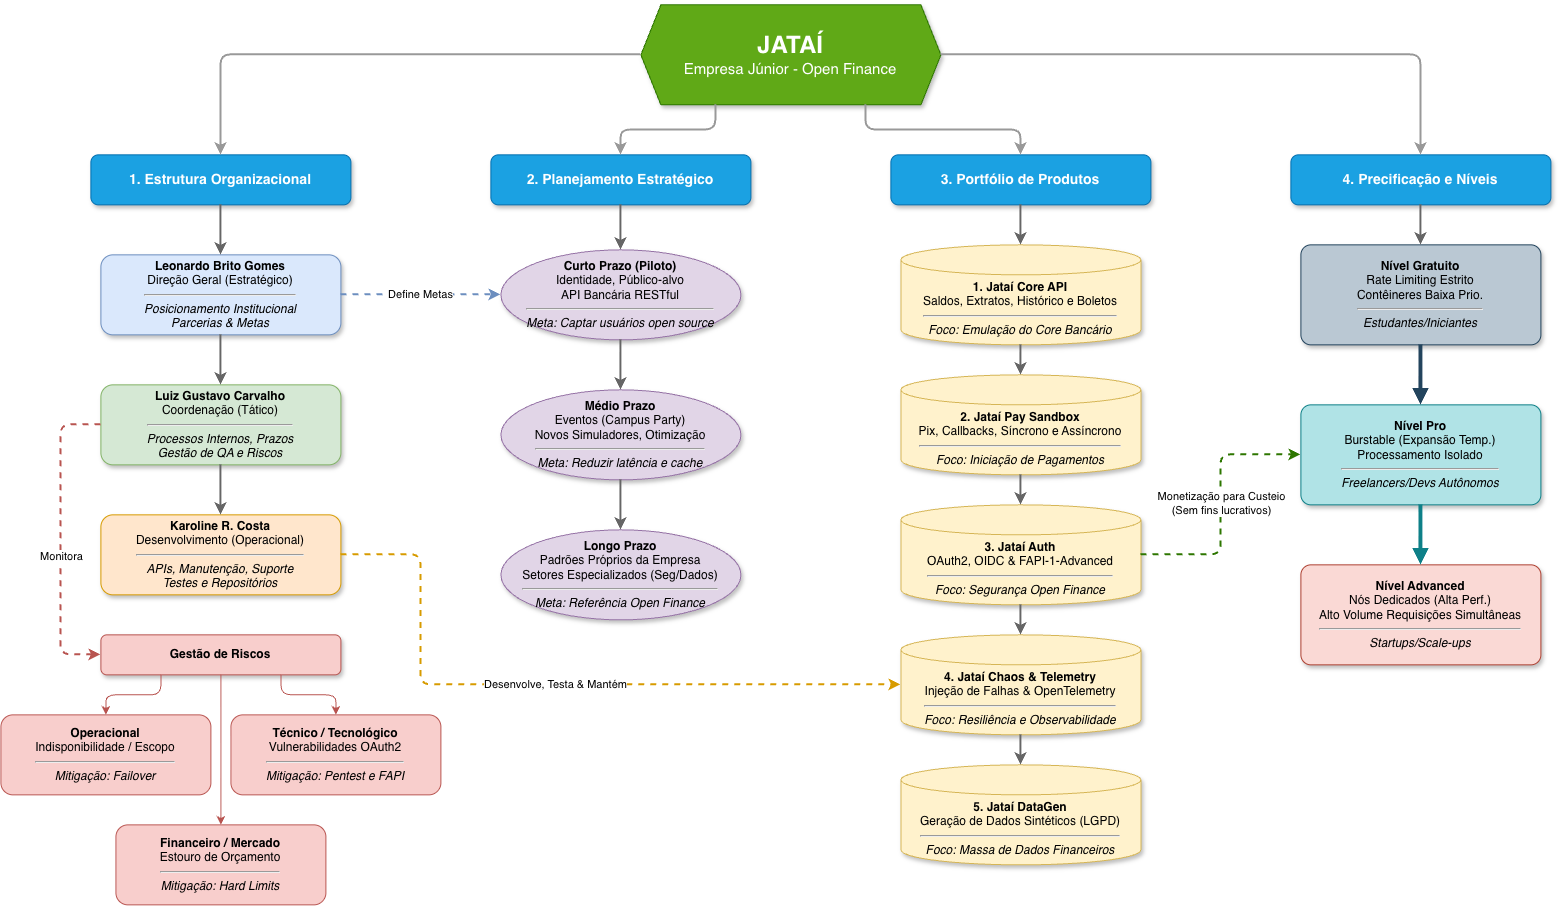
\includegraphics[width=0.6\textwidth]{organograma_jatai.png}
    \caption{Mapa estratégico, estrutura organizacional e matriz de produtos da Jataí.}
    \label{fig:organograma_jatai}
    \legend{Fonte: Elaborado pelos autores (2026).}
\end{figure}

O modelo visual consolida a relação de subordinação e cooperação técnica entre os membros, além de mapear diretamente a atuação do nível tático sobre o controle de riscos e a supervisão contínua da entrega do portfólio de \textit{software}.

\section{Descrição das funções e cargos}
\label{sec:descricao_cargos}

A alocação dos membros reflete as competências requeridas para a sustentabilidade institucional e o desenvolvimento técnico do ecossistema de simulação. As atribuições e responsabilidades formais de cada cargo são detalhadas a seguir.

\subsection{Direção geral (nível estratégico)}
{Responsável:} Leonardo Brito. {Escopo de Atuação:} Governança Institucional, Relações Governamentais e Planejamento Estratégico. O Diretor Geral ocupa o topo da cadeia decisória da Jataí, sendo o principal responsável por assegurar a aderência da empresa júnior aos seus fins estatutários e à legislação vigente.
\begin{itemize}
    \item Atribuições Principais:
    \begin{itemize}
        \item Definir o posicionamento estratégico e a visão de longo prazo da empresa no mercado de tecnologia bancária;
        \item Prospectar parcerias institucionais, convênios acadêmicos e parcerias com o ecossistema \textit{open-source};
        \item Determinar as metas globais de crescimento, sustentabilidade financeira e expansão do portfólio;
        \item Representar formalmente a empresa perante órgãos reguladores, instâncias universitárias e contratantes.
    \end{itemize}
    \item Entregáveis: Plano de negócios trienal, acordos de parceria institucional, relatórios globais de desempenho.
\end{itemize}

\subsection{Coordenação de operações, QA e riscos (nível tático)}
{Responsável:} Luiz Gustavo. {Escopo de atuação:} gestão de processos, garantia da qualidade (Quality Assurance) e gestão de riscos.

O Coordenador atua como a ponte de ligação entre o direcionamento estratégico e a execução técnica. Responde pelo cumprimento dos prazos, alocação de recursos e supervisão transversal da segurança e estabilidade operacional.
\begin{itemize}
    \item{Atribuições principais:}
    \begin{itemize}
        \item Gerenciar o cronograma de entregas, metodologias ágeis (Scrum/Kanban) e marcos operacionais do projeto;
        \item Coordenar as rotinas de Quality Assurance (QA), definindo os critérios de aceite e padrões de código;
        \item Monitorar e mitigar ativamente os riscos mapeados (Operacionais, Tecnológicos/Segurança e Financeiros);
        \item Implementar planos de contingência, como procedimentos de failover, protocolos de resposta a incidentes e controle de Hard Limits orçamentários.
    \end{itemize}
    \item Entregáveis: matriz de riscos atualizada, matriz de rastreabilidade de QA, relatórios de desempenho operacional e SLAs.
\end{itemize}

\subsection{Engenharia de desenvolvimento e manutenção (nível operacional)}
{Responsável:} Karoline Costa. {Escopo de atuação:} arquitetura de software, desenvolvimento de APIs, testes e infraestrutura DevOps.

A Engenheira de Desenvolvimento responde pela construção efetiva das soluções tecnológicas, manutenção dos repositórios e garantia do correto funcionamento das interfaces programáticas.
\begin{itemize}
    \item Atribuições principais:
    \begin{itemize}
        \item Projetar, codificar e manter os componentes do portfólio (Jataí Core API, Pay Sandbox, Jataí Auth, Chaos \& Telemetry, DataGen);
        \item Escrever e executar suítes de testes unitários, de integração e de estresse para garantir conformidade com os perfis de segurança FAPI e OAuth2;
        \item Prestar suporte técnico, gerenciar commits, pull requests e documentar detalhadamente os endpoints RESTful nos repositórios oficiais;
        \item Configurar pipelines de CI/CD, contêineres de simulação e rotinas de telemetria.
    \end{itemize}
    \item Entregáveis: código-fonte do ecossistema, suítes de testes automatizados, documentação Swagger/OpenAPI, repositórios Git atualizados.
\end{itemize}

\section{Matriz de responsabilidades (RACI)}
\label{sec:matriz_raci}

Para evitar superposição de papéis e assegurar o cumprimento rigoroso dos fluxos operacionais, a Tabela~\ref{tab:matriz_raci} estabelece a Matriz RACI (\textit{Responsible, Accountable, Consulted, Informed}) para os principais processos da organização.

\begin{table}[htbp]
\centering
\caption{Matriz de responsabilidade RACI para processos da Jataí.}
\label{tab:matriz_raci}
\resizebox{\textwidth}{!}{
\begin{tabular}{|l|c|c|c|}
\hline
\textbf{Processo / Atividade} & \textbf{Direção Geral} & \textbf{Coordenação} & \textbf{Desenvolvimento} \\ \hline
Definição de Parcerias e Metas Estratégicas & \textbf{A / R} & C & I \\ \hline
Aprovação do Cronograma e Prazos & I & \textbf{A / R} & C \\ \hline
Arquitetura e Implementação de APIs & I & C & \textbf{A / R} \\ \hline
Homologação de Código e Testes de QA & I & \textbf{A} & \textbf{R} \\ \hline
Gestão e Mitigação de Riscos de Segurança & C & \textbf{A / R} & C \\ \hline
Suporte Técnico e Resolução de BUGS & I & C & \textbf{A / R} \\ \hline
\end{tabular}
}
\legend{Legenda: \textbf{R}: Responsável executor (\textit{Responsible}); \textbf{A}: Aprovador/Prestador de contas (\textit{Accountable}); \textbf{C}: Consultado (\textit{Consulted}); \textbf{I}: Informado (\textit{Informed}). Fonte: Elaborado pelos autores (2026).}
\end{table}


\chapter{Recursos humanos}
\label{cap:recursos_humanos}

A política de gestão de pessoas fundamenta-se no desenvolvimento do capital humano acadêmico, associando a formação técnica em computação/TI e \textit{Open Finance} ao cultivo de competências comportamentais e de liderança. Em conformidade com a Lei nº 13.267/2016, a empresa opera como uma incubadora de talentos, garantindo a renovação contínua de seus quadros através de processos seletivos e programas estruturados de capacitação.

\section{Dimensionamento e projeção do quadro de colaboradores}
\label{sec:dimensionamento_quadro}

A composição da equipe foi dimensionada com base nas demandas de desenvolvimento, suporte, governança e conformidade regulatória. Atualmente composta por 3 (três) membros fundadores, a estrutura prevê uma expansão gradual ao longo dos ciclos operacionais para absorver a evolução do portfólio de produtos e assegurar a redundância operacional.

A Tabela~\ref{tab:projecao_quadro} apresenta a evolução estimada do quadro de colaboradores por nível de atuação e área funcional ao longo dos horizontes de curto, médio e longo prazo.

\begin{table}[htbp]
\centering
\caption{Projeção de evolução do quadro de colaboradores da Jataí.}
\label{tab:projecao_quadro}
\resizebox{\textwidth}{!}{
\begin{tabular}{|l|l|c|c|c|}
\hline
\textbf{Nível Hierárquico} & \textbf{Função / Área} & \textbf{Atual (Piloto)} & \textbf{Médio Prazo} & \textbf{Longo Prazo} \\ \hline
Estratégico & Direção Geral / Institucional & 1 & 1 & 2 \\ \hline
Tático & Coordenação de Operações, QA e Riscos & 1 & 2 & 3 \\ \hline
Operacional & Engenharia de APIs e Backend & 1 & 3 & 5 \\ \hline
Operacional & Segurança, Identity \& FAPI & 0 & 1 & 2 \\ \hline
Operacional & Telemetria, DevOps \& Dados & 0 & 1 & 2 \\ \hline
Formação & Trainees / Estagiários em Imersão & 0 & 2 & 4 \\ \hline
\textbf{Total Geral} & & \textbf{3} & \textbf{10} & \textbf{18} \\ \hline
\end{tabular}
}
\legend{Fonte: Elaborado pelos autores (2026).}
\end{table}

A expansão do quadro operacional visa mitigar o risco de ponto único de falha (\textit{Single Point of Failure - SPOF}) no desenvolvimento técnico e permitir o escalonamento das atividades de testes de carga e monitoramento das APIs bancárias.

\section{Processo de Admissão}
\label{sec:processo_selecao}

O Processo seletivo é conduzido semestralmente e estruturado em 5 (cinco) etapas eliminatórias e classificatórias, desenhado para avaliar simultaneamente a capacidade de resolução de problemas, a base técnica e o alinhamento com os valores institucionais da empresa.

\begin{enumerate}[label={Etapa \arabic*:}]
    \item{Inscrição e triagem curricular:} análise do histórico acadêmico, pré-requisitos matriciais na instituição de ensino superior e preenchimento do formulário de intenção motivacional.
    \item{Dinâmica de grupo e fit cultural:} avaliação de competências socioemocionais (soft skills), tais como comunicação, trabalho em equipe, ética, proatividade e alinhamento com o ecossistema de empreendedorismo acadêmico.
    \item{Desafio técnico (Hackathon / estudo de caso):} resolução de um problema prático simplificado de arquitetura de software ou modelagem de dados RESTful. Avalia a raciocínio lógico, capacidade de pesquisa, conceitos básicos de Git e higiene de código.
    \item{Entrevista estruturada por competências:} entrevista individual conduzida pela Direção e Coordenação para validação do compromisso com a carga horária semanal, expectativas de carreira e aprofundamento das respostas técnicas.
    \item{Programa trainee (imersão onboarding):} período de 4 semanas de ambientação em que o candidato aprovado realiza miniprojetos supervisionados antes da efetivação no quadro regular.
\end{enumerate}

\section{Sistema de avaliação de desempenho}
\label{sec:avaliacao_desempenho}

Para assegurar a excelência nas entregas técnicas e o crescimento profissional contínuo dos integrantes, a Jataí adota um modelo híbrido de avaliação de desempenho composto por três eixos de mensuração:

\subsection{Matriz de competências}
A cada final de ciclo semestral, o colaborador é avaliado quanto ao domínio de habilidades essenciais para a sua função.
\begin{itemize}
    \item{Competências técnicas (hard skills):} domínio de padrões RESTful, segurança OAuth2/FAPI, escrita de testes automatizados, controle de versão e documentação de APIs;
    \item{Competências comportamentais (soft skills):} cumprimento de prazos, pontualidade, clareza na comunicação interna, capacidade de dar e receber feedbacks e atitude colaborativa.
\end{itemize}

\subsection{Acompanhamento por OKRs (\textit{Objectives and Key Results})}
As metas individuais e de equipe são vinculadas aos OKRs operacionais da organização. Cada integrante possui metas objetivas e quantificáveis, tais como:
\begin{itemize}
    \item Manutenção da cobertura de testes unitários em nível superior a $85\%$;
    \item Redução do tempo médio de resolução de chamados ou \textit{bugs} (\textit{Mean Time to Repair - MTTR});
    \item Cumprimento de $100\%$ das entregas alocadas no \textit{sprint backlog}.
\end{itemize}

\subsection{Avaliação 360 Graus e rituais de feedback}
O processo encerra-se com a autoavaliação do colaborador, a avaliação pelos pares e a avaliação da liderança. Os resultados são consolidados na matriz $9$-Box (Desempenho x Potencial), orientando as decisões de promoção interna, recondução de cargos e correções de rota.

\section{Plano de Desenvolvimento dos Integrantes (PDI)}
\label{sec:plano_desenvolvimento}

O Plano de Desenvolvimento Individual (PDI) é o instrumento estratégico que alinha as aspirações de carreira do estudante às necessidades de maturidade tecnológica do projeto. Todo integrante aprovado constrói seu PDI junto à coordenação no início de cada gestão. O plano é estruturado em duas matrizes de capacitação contínua:

\subsection{Trilha de engenharia e Open Finance}
\begin{itemize}
    \item{Módulo 1 — Fundamentos de Open Finance:} Arquitetura do \bcb{}, APIs de Consentimento, Perfis FAPI-1-Advanced e LGPD aplicada ao setor financeiro;
    \item{Módulo 2 — Arquitetura de Microsserviços:} Modelagem RESTful, resiliência, padrões de concorrência e conteinerização com Docker;
    \item{Módulo 3 — Qualidade e Telemetria:} Testes funcionais e de estresse, integração contínua (CI/CD) e instrumentação com OpenTelemetry.
\end{itemize}

\subsection{Trilha de liderança e governança}
\begin{itemize}
    \item{Módulo 1 — Gestão Ágil:} Framework Scrum, gestão de \textit{backlog} e priorização técnica;
    \item{Módulo 2 — Governança de Riscos:} Mapeamento e mitigação de riscos operacionais, segurança cibernética e \textit{compliance};
    \item{Módulo 3 — Comunicação Técnica:} Redação de documentação arquitetural, relatórios de auditoria e mentoria de novos membros.
\end{itemize}

\vspace{0.5em}
Além das trilhas assíncronas e treinamentos internos, a Jataí fomenta a participação dos colaboradores em eventos acadêmicos, seminários sobre o ecossistema financeiro e maratonas de programação.

\chapter{Análise de mercado}
\section{Público-alvo}
Nosso público-alvo principal são estudantes de tecnologia que buscam alternativas para iniciar o desenvolvimento de integrações com o sistemas bancários ou que buscam otimizar suas aplicações. A utilização simultânea dos 5 produtos que disponibilizamos tem como objetivo atrair um pública que precisa de um ambiente sandbox para simular transações bancárias.

\section{Concorrentes}
Os principais concorrentes relacionados a nossa proposta são Sandboxes de bancos e fintechs, Ferramentas genéricas de mock de APIs e Projetos open source de Open Banking. Cada uma dessas soluções possui suas vantagens de desvantagens, porém nenhuma delas possui como foco principal fornecer um ecossistema financeiro simulado, integrado e de fácil instalação voltado para aprendizado e prototipação.

\subsection{Sandboxes de bancos e fintechs}
Os sandboxes disponibilizados por bancos e fintechs possuem mecanismos robustos de segurança e documentação detalhada, a inscrição no Portal de Desenvolvedores do Banco do Brasil pode possibilitar a utilização de um fluxo para publicação de integrações testadas em homologação para produção caso os requisitos de uso da API em específico sejam atendidos \parencite{docBB}.

Em geral, o objetivo desses ambientes é simular a integração com o provedor em específico, simulando inclusive a sua forma própria de segurança de APIs, além disso, não é permitida a execução de uma instância própria da API pelo usuário.

\subsection{Ferramentas genéricas de mock de APIs}
As ferramentas de mock de APIs como o Postman \parencite{postmanMockDoc} possibilitam o usuário gerar uma instância própria da API em sua máquina local, mas não simulam um banco. Seu intuito é a criação de APIs genéricas, isso significa que o usuário terá que manualmente, desenvolver o comportamento que ele espera daquela API simulada enquanto nossa solução segue uma filosofia de ``\textit{plug and play}'' onde, ao subir os produtos que disponibilizamos localmente, o usuário já consegue uma simulação de sistema bancário pronta.

\subsection{Projetos open source de Open Banking}
Projetos como o Open Bank Project \parencite{opbApi} possuem uma proposta próxima ao desenvolvimento de APIs bancárias abertas, disponibilizando uma plataforma open source para implementação de serviços financeiros.

Entretanto, o projeto possui como principal objetivo atender instituições e organizações interessadas em construir ou experimentar soluções de Open Banking, possuindo uma complexidade de configuração e operação mais adequada para ambientes profissionais.

A solução proposta busca atender uma necessidade diferente, oferecendo um ambiente simplificado, com instalação facilitada e foco educacional, permitindo que estudantes e desenvolvedores possam experimentar conceitos financeiros por meio de uma infraestrutura local e integrada.

\section{Parceiros e fornecedores}
Nossa solução depende de uma rede de parceiros estratégicos e fornecedores de infraestrutura de nuvem para garantir seu desenvolvimento, adoção e manutenção. Para manter a proposta de fornecer um ambiente pronto para quem não quer utilizar o serviço com self-hosting, o Jataí se propõe a utilizar serviços em nuvem nas versões pagas de cada serviço, onde a arrecadação do serviço tem como finalidade apenas custear a infraestrutura necessária para manutenção da plataforma, em conformidade com o caráter sem fins lucrativos das empresas juniores.

\subsection{Parceiros}
A natureza open source do projeto permite que a comunidade contribua com ideias, melhorias e novas funcionalidades. Os principais parceiros da Jataí são:

\begin{itemize}
    \item{Instituições de ensino e professores orientadores}: utilização da plataforma em disciplinas, projetos de pesquisa, extensão e empresas juniores, contribuindo para a formação prática de estudantes.
    
    \item{Comunidades de tecnologia}: grupos de usuários, comunidades open source, hackathons e eventos técnicos podem contribuir para divulgação da plataforma, recebimento de feedback e evolução dos produtos.
    
    \item{Bancos, fintechs e cooperativas de crédito}: parcerias voltadas à validação dos fluxos simulados, identificação de boas práticas e aproximação entre o ambiente acadêmico e o mercado financeiro.
    
    \item{Empresas de infraestrutura em nuvem}: provedores como AWS, Google Cloud Platform e Microsoft Azure podem fornecer infraestrutura para a versão hospedada da plataforma, além de programas de créditos para startups e projetos educacionais.
\end{itemize}

\subsection{Fornecedores}
Para disponibilizar a solução em nuvem, o Jataí utilizará serviços de provedores como AWS e Google Cloud, que oferecem serviços de hospedagem, banco de dados e gerenciamento de contêineres. A escolha desses fornecedores se baseia na confiabilidade, escalabilidade e suporte técnico oferecidos por essas plataformas, garantindo que os usuários tenham acesso a um ambiente estável e seguro para suas atividades de aprendizado e prototipagem.

Como nossa solução foi pensada como algo portátil e flexível, a escolha de provedores de nuvem não é restritiva, podendo ser alterada conforme a necessidade, desde que os requisitos técnicos sejam atendidos. Apesar disso, demonstramos preferência pela AWS por ser uma das principais fornecedoras de infraestrutura em nuvem devido à ampla oferta de serviços em nuvem, alta disponibilidade, escalabilidade e grande quantidade de documentação técnica disponível \parencite{awsDoc}.

\section{Oportunidades e ameaças}
Como oportunidades temos a demanda por profissionais capacitados em integração de sistemas financeiros, a crescente adoção do Open Finance no Brasil, a possibilidade de parcerias estratégicas com instituições de ensino e empresas do setor financeiro, além da expansão do mercado de tecnologia e inovação. Essas oportunidades podem impulsionar o crescimento da Jataí, permitindo que ela se torne uma referência na formação técnica voltada ao desenvolvimento de soluções para o ecossistema financeiro.

Como ameaças, podemos citar a concorrência de sandboxes de bancos e fintechs, a complexidade regulatória do setor financeiro, a rápida evolução das tecnologias e especificações do ecossistema financeiro e a necessidade de atualização constante dos conteúdos e ferramentas oferecidas pela Jataí. Além disso, a dependência de provedores de infraestrutura em nuvem podem revelar um desafio para manutenção da disponibilidade da aplicação por meio de alterações nos custos operacionais ou baixa adesão dos planos pagos.

\section{Parcerias estratégicas}
A parceria com instituições de ensino e professores orientadores pode ser uma oportunidade estratégica de divulgação da solução, permitindo que a plataforma seja incorporada em disciplinas, projetos de pesquisa e extensão, além de empresas juniores. Essa colaboração pode gerar feedback valioso para aprimorar os produtos e adaptar a plataforma às necessidades educacionais.

Outra parceria estratégica envolve a colaboração com comunidades de tecnologia de forma geral. Essa colaboração pode gerar, além da divulgação da plataforma, a possibilidade de receber feedbacks e melhorias da comunidade através de \textit{forks} e \textit{pull requests}. Além disso, pode possibilitar a realização de hackathons e eventos técnicos que promovam o uso da plataforma e incentivem a inovação.
Por fim, parcerias com bancos, fintechs e cooperativas de crédito podem contribuir para a validação dos fluxos financeiros simulados e para a aproximação da plataforma com práticas adotadas pelo mercado. Essa colaboração possibilita que as simulações permaneçam alinhadas às tecnologias e aos padrões utilizados em ambientes reais, aumentando a relevância da solução para estudantes e desenvolvedores.

\chapter{Portfólio de produtos e serviços}
\label{cap:portfolio_produtos}

A Jataí oferece simuladores e ferramentas de infraestrutura para desenvolvedores, \textit{fintechs} e pesquisadores do ecossistema de \textit{Open Finance}. O portfólio é estruturado em três categorias funcionais complementares: Simulação Bancária Core, Segurança e Identidade, e Infraestrutura, Testes e Dados.

\section{Categoria 1 - produtos de simulação bancária}
\label{sec:cat_simulacao_bancaria}

\subsection{Jataí Core API}
\label{subsec:jatai_core_api}

O Jataí Core API consiste em um servidor RESTful destinado à simulação das principais operações bancárias. A solução replica fielmente as respostas e os schemas de payload utilizados no ecossistema Open Finance Brasil, permitindo a consulta de saldo, extrato e histórico de transações, além da emissão simulada de cobranças e boletos. Seu público-alvo é composto por desenvolvedores front-end e mobile, projetistas de interfaces e estudantes de engenharia de software que necessitam de um ambiente confiável para desenvolvimento e experimentação. A plataforma foi concebida para suprir a indisponibilidade de APIs bancárias de produção durante as etapas de desenvolvimento e homologação, bem como a escassez de dados financeiros estruturados para validação de interfaces de usuário. Como resultado, proporciona redução do tempo de prototipagem de aplicações financeiras, disponibiliza um ambiente gratuito e independente de instituições financeiras reais e oferece integração nativa com o módulo Jataí Pay Sandbox.

\begin{figure}[htbp]
\centering
\caption{Representação das rotas e payload da interface do Jataí Core API.}
\label{fig:jatai_core_api}

\begin{tabular}{|l|l|l|p{4cm}|}
\hline
\textbf{Método} & \textbf{Endpoint} & \textbf{Status} & \textbf{Descrição} \\ \hline
\texttt{GET} & \texttt{/api/v1/accounts/\{id\}/balance} & 200 OK & Saldo Atual \\ \hline
\texttt{GET} & \texttt{/api/v1/accounts/\{id\}/statement} & 200 OK & Extrato Transacional \\ \hline
\texttt{POST} & \texttt{/api/v1/bank-slips/generate} & 201 Created & Emissão de Boleto \\ \hline
\end{tabular}

\vspace{0.8em}

\begin{minipage}{0.75\textwidth}
\begin{lstlisting}[language=json, caption={Exemplo de payload de resposta (JSON)}]
{
  "account": "10023-9",
  "balance": 4500.00,
  "currency": "BRL"
}
\end{lstlisting}
\end{minipage}

\legend{Fonte: Elaborado pelos autores (2026).}
\end{figure}

\subsection{Jataí Pay Sandbox}
\label{subsec:jatai_pay_sandbox}

O Jataí Pay Sandbox consiste em um ambiente isolado e seguro destinado à simulação de requisições de Iniciação de Pagamento Instantâneo (Pix). A plataforma permite a emulação completa de fluxos síncronos e assíncronos por meio de webhooks e callbacks, oferecendo um ambiente controlado para validação de integrações. Seu público-alvo é composto por desenvolvedores back-end, integradores de gateways de pagamento e fintechs em fase de homologação. A solução foi concebida para reduzir os riscos financeiros e a complexidade operacional associados aos testes de transações de pagamento em ambientes bancários tradicionais de homologação. Entre seus principais benefícios estão a possibilidade de testar fluxos de liquidação instantânea sem movimentação de valores reais, validar a resiliência das aplicações diante de falhas no recebimento de callbacks e cobrir integralmente cenários de sucesso, rejeição e tempo limite (timeout).

\begin{figure}[htbp]
\centering
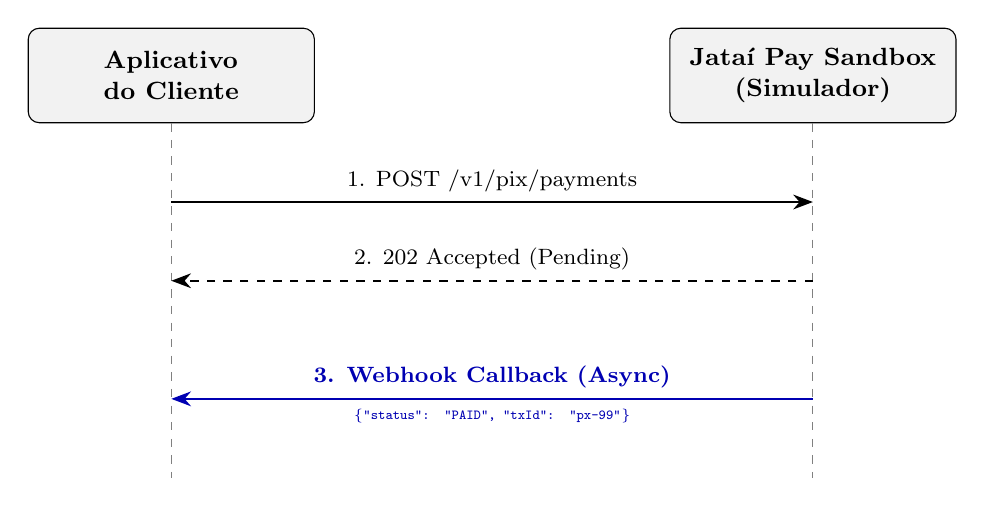
\begin{tikzpicture}[
    node distance=4.5cm,
    auto,
    block/.style={rectangle, draw, fill=gray!10, text width=3.4cm, text centered, rounded corners, minimum height=1.2cm, font=\bfseries\small},
    line/.style={draw, -{Stealth[length=2.5mm]}, thick},
    dashedline/.style={draw, -{Stealth[length=2.5mm]}, thick, dashed}
]

    \node [block] (client) {Aplicativo do Cliente};
    \node [block, right=of client] (sandbox) {Jataí Pay Sandbox\\(Simulador)};

    \draw [gray, dashed] (client.south) -- ([yshift=-4.5cm]client.south);
    \draw [gray, dashed] (sandbox.south) -- ([yshift=-4.5cm]sandbox.south);

    \draw [line] ([yshift=-1.0cm]client.south) -- node[above, font=\footnotesize] {1. POST /v1/pix/payments} ([yshift=-1.0cm]sandbox.south);

    \draw [dashedline] ([yshift=-2.0cm]sandbox.south) -- node[above, font=\footnotesize] {2. 202 Accepted (Pending)} ([yshift=-2.0cm]client.south);

    \draw [line, color=blue!70!black] ([yshift=-3.5cm]sandbox.south) -- node[above, font=\footnotesize\bfseries] {3. Webhook Callback (Async)} node[below, font=\ttfamily\tiny] {\{"status": "PAID", "txId": "px-99"\}} ([yshift=-3.5cm]client.south);

\end{tikzpicture}
\caption{Fluxo de comunicação assíncrona e retorno via Webhook no Jataí Pay Sandbox.}
\label{fig:jatai_pay_sandbox}
\legend{Fonte: Elaborado pelos autores (2026).}
\end{figure}

\section{Categoria 2 - produtos de segurança e identidade}
\label{sec:cat_seguranca_identidade}

\subsection{Jataí Auth}
\label{subsec:jatai_auth}

O Jataí Auth consiste em um provedor de identidade e servidor de autorização desenvolvido com base nos protocolos OAuth 2.0 e OpenID Connect (OIDC), em conformidade com o perfil de segurança Financial-grade API (FAPI-1-Advanced). A solução é destinada a arquitetos de software, especialistas em segurança cibernética e equipes de desenvolvimento back-end que necessitam implementar mecanismos seguros de autenticação e autorização em aplicações voltadas ao ecossistema Open Finance. A plataforma foi concebida para reduzir a complexidade de configuração e o elevado custo inicial de implementação das camadas de autenticação e gestão de escopos de consentimento exigidas pelo Open Finance. Entre seus principais benefícios estão a validação imediata de trocas de tokens (JWT), PKCE e assinaturas digitais, a disponibilização de ambientes pré-configurados para simulação de telas de consentimento do usuário e a simplificação da conformidade regulatória em projetos que se encontram em estágio de prova de conceito.

\begin{figure}[htbp]
\centering
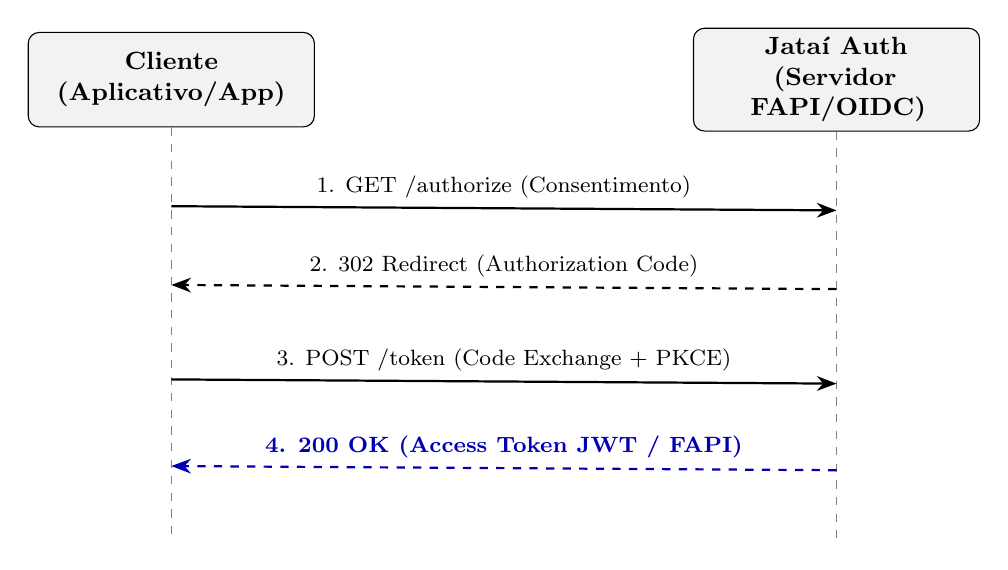
\begin{tikzpicture}[
    node distance=4.8cm,
    auto,
    block/.style={rectangle, draw, fill=gray!10, text width=3.4cm, text centered, rounded corners, minimum height=1.2cm, font=\bfseries\small},
    line/.style={draw, -{Stealth[length=2.5mm]}, thick},
    dashedline/.style={draw, -{Stealth[length=2.5mm]}, thick, dashed}
]

    \node [block] (client) {Cliente\\(Aplicativo/App)};
    \node [block, right=of client] (auth) {Jataí Auth\\(Servidor FAPI/OIDC)};

    \draw [gray, dashed] (client.south) -- ([yshift=-5.2cm]client.south);
    \draw [gray, dashed] (auth.south) -- ([yshift=-5.2cm]auth.south);

    \draw [line] ([yshift=-1.0cm]client.south) -- node[above, font=\footnotesize] {1. GET /authorize (Consentimento)} ([yshift=-1.0cm]auth.south);

    \draw [dashedline] ([yshift=-2.0cm]auth.south) -- node[above, font=\footnotesize] {2. 302 Redirect (Authorization Code)} ([yshift=-2.0cm]client.south);

    \draw [line] ([yshift=-3.2cm]client.south) -- node[above, font=\footnotesize] {3. POST /token (Code Exchange + PKCE)} ([yshift=-3.2cm]auth.south);

    \draw [dashedline, color=blue!70!black] ([yshift=-4.3cm]auth.south) -- node[above, font=\footnotesize\bfseries] {4. 200 OK (Access Token JWT / FAPI)} ([yshift=-4.3cm]client.south);

\end{tikzpicture}
\caption{Diagrama de concessão de autorização e emissão de Token no Jataí Auth.}
\label{fig:jatai_auth}
\legend{Fonte: Elaborado pelos autores (2026).}
\end{figure}

\section{Categoria 3 - produtos de infraestrutura, testes e dados}
\label{sec:cat_infra_dados}

\subsection{Jataí Chaos \& Telemetry}
\label{subsec:jatai_chaos_telemetry}

O Jataí Chaos \& Telemetry consiste em uma suíte de instrumentação e injeção de falhas destinada à análise de desempenho de aplicações. A solução monitora, em tempo real, métricas como tempo de resposta, latência e taxa de erro, além de permitir a simulação de degradação de rede e sobrecarga de requisições. Seu público-alvo é composto por engenheiros de Site Reliability (SRE), testadores de carga e desenvolvedores DevOps que necessitam avaliar a resiliência e o desempenho de sistemas distribuídos. A plataforma foi desenvolvida para facilitar a identificação de gargalos arquiteturais e o diagnóstico do comportamento de aplicações em cenários adversos de instabilidade de APIs de terceiros. Entre seus principais benefícios destacam-se a identificação precoce de problemas de desempenho e consultas ineficientes, a simulação de cenários de Chaos Engineering e a emissão de relatórios e métricas compatíveis com o padrão OpenTelemetry.

\begin{figure}[htbp]
\centering
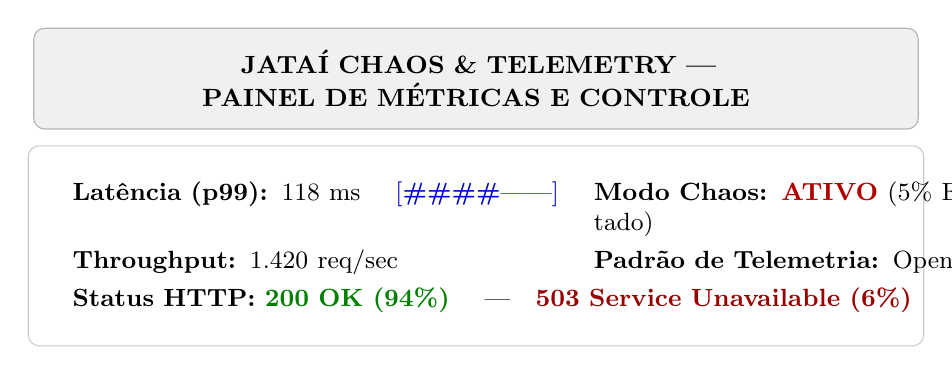
\begin{tikzpicture}[
    node distance=0.4cm,
    auto
]
    \node[draw=gray!60, fill=gray!12, rounded corners=4pt, inner sep=8pt, text width=0.88\textwidth, align=center] (header) {
        \bfseries\small JATAÍ CHAOS \& TELEMETRY --- PAINEL DE MÉTRICAS E CONTROLE
    };

    \node[draw=gray!40, fill=white, rounded corners=4pt, inner sep=10pt, text width=0.88\textwidth, below=0.2cm of header] (metrics) {
        \small
        \begin{tabular}{p{6.2cm} p{6.2cm}}
            \textbf{Latência (p99):} 118 ms \quad \textcolor{blue!80!black}{[\textbf{\#\#\#\#}------]} & \textbf{Modo Chaos:} \textcolor{red!70!black}{\textbf{ATIVO}} (5\% Erro Injetado) \\
            \textbf{Throughput:} 1.420 req/sec & \textbf{Padrão de Telemetria:} OpenTelemetry \\
            \multicolumn{2}{l}{\textbf{Status HTTP:} \textcolor{green!50!black}{\textbf{200 OK (94\%)}} \quad|\quad \textcolor{red!60!black}{\textbf{503 Service Unavailable (6\%)}}}
        \end{tabular}
    };
\end{tikzpicture}
\caption{Painel de telemetria e controle de injeção de falhas do Jataí Chaos \& Telemetry.}
\label{fig:jatai_chaos_telemetry}
\legend{Fonte: Elaborado pelos autores (2026).}
\end{figure}

\subsection{Jataí DataGen}
\label{subsec:jatai_datagen}

O Jataí DataGen consiste em um motor algorítmico parametrizável desenvolvido para a geração em larga escala de dados financeiros sintéticos, relacionais e anonimizados. A solução é destinada a cientistas de dados, engenheiros de Machine Learning e equipes de garantia da qualidade (QA), oferecendo um ambiente adequado para desenvolvimento, testes e treinamento de modelos computacionais. A plataforma foi concebida para suprir a escassez de bases de dados realistas e contornar as restrições legais impostas pela LGPD quanto ao uso de dados pessoais reais em ambientes de desenvolvimento e treinamento de modelos de inteligência artificial. Entre seus principais benefícios destacam-se a geração de volumes configuráveis de dados em conformidade com a legislação vigente, a preservação das propriedades estatísticas e das correlações financeiras necessárias ao treinamento de modelos de IA e a exportação simplificada dos conjuntos de dados em múltiplos formatos, como JSON, CSV e SQL.

\begin{figure}[htbp]
\centering
\caption{Estrutura do payload de dados sintéticos gerado pelo Jataí DataGen.}
\label{fig:jatai_datagen}

\begin{minipage}{0.85\textwidth}
\begin{lstlisting}[language=json, caption={Exemplo de Payload Sintético Anonimizado (Conformidade LGPD)}]
{
  "synthetic_user_id": "syn-usr-9941",
  "holder_name": "Anonimizado_0481",
  "credit_score": 780,
  "transactions_30d": [
    {
      "type": "PIX",
      "amount": 150.00
    }
  ]
}
\end{lstlisting}
\end{minipage}

\legend{Fonte: Elaborado pelos autores (2026).}
\end{figure}

\section{Níveis de acesso e modelo de precificação}
\label{sec:niveis_precificacao}

Para garantir a autossustentabilidade da empresa (lembrando do aspecto de ser sem fins lucrativos), o acesso ao ecossistema Jataí é oferecido em três níveis de serviço. Os valores foram dimensionados utilizando a calculadora de custos de infraestrutura em nuvem da AWS (\textit{AWS Pricing Calculator}), cobrindo custos fixos de processamento em contêineres (Amazon EC2) e armazenamento de dados relacionais (Amazon RDS). A Tabela~\ref{tab:niveis_precificacao} detalha a estrutura de planos e seus respectivos públicos-alvo.

\begin{table}[htbp]
\centering
\caption{Matriz de níveis de acesso, precificação e perfil de infraestrutura.}
\label{tab:niveis_precificacao}
\resizebox{\textwidth}{!}{
\begin{tabular}{|c|p{5.5cm}|c|p{4.5cm}|}
\hline
\textbf{Nível} & \textbf{Descrição da Infraestrutura} & \textbf{Preço Estimado} & \textbf{Público-Alvo} \\ \hline

\textbf{Gratuito} &
Acesso total ao código-fonte (\textit{Open Source}) para execução local (\textit{Self-hosted}) via Docker. Sujeito a \textit{rate limiting} estrito nas instâncias públicas de teste. &
R\$ 0,00 &
Estudantes, pesquisadores acadêmicos e desenvolvedores em aprendizado. \\ \hline

\textbf{Pro} &
Ambiente em nuvem gerenciado, com capacidade elástica (\textit{burstable}) e execução isolada de contêineres. Disponibilidade operacional garantida em horário comercial. &
R\$ 19,90 / mês &
Desenvolvedores autônomos, \textit{freelancers} e pequenas equipes de desenvolvimento. \\ \hline

\textbf{Advanced} &
Nós dedicados de alta performance na nuvem, com suporte a alto volume de requisições simultâneas, simulação avançada de caos e relatórios customizados. &
R\$ 89,90 / mês &
\textit{Startups}, \textit{fintechs} em estágio inicial e laboratórios de inovação corporativa. \\ \hline

\end{tabular}
}
\legend{Fonte: Elaborado pelos autores (2026).}
\end{table}

\chapter{Plano de marketing}
\label{cap:plano_marketing}

O Plano de Marketing adota a abordagem de \textit{Developer Relations} (DevRel) e Marketing Orientado a Produto (\textit{Product-Led Growth} - PLG). Considerando que o público-alvo da empresa é composto por desenvolvedores, arquitetos de \textit{software}, pesquisadores e fintechs, a estratégia de comunicação prioriza a utilidade técnica, a excelência funcional das ferramentas e a presença ativa em fóruns de capacitação, em detrimento do marketing B2C tradicional.

\section{Identidade visual e conceito da marca}
\label{sec:identidade_visual}

A identidade visual da empresa inspira-se na \textit{Tetragonisca angustula}, popularmente conhecida como abelha Jataí — uma espécie nativa brasileira sem ferrão, reconhecida por sua agilidade, organização em colônia, arquitetura de favos resilientes e produção de alto valor agregado.

\subsection{Simbologia e elementos}
A metáfora da abelha Jataí conecta-se diretamente aos princípios do \textit{Open Finance} e do desenvolvimento de \textit{software} moderno:
\begin{itemize}
    \item{Colaboração e descentralização:} assim como uma colônia de Jataís funciona de forma orquestrada sem centralização rígida, as APIs do Open Finance conectam múltiplos nós de um ecossistema financeiro aberto;
    \item{Arquitetura em favo (hexagonal):} o favo de mel representa a arquitetura de software modular (arquitetura hexagonal / Ports and Adapters), simbolizando resiliência, organização e encaixe perfeito entre microsserviços;
    \item{Agilidade e segurança sem conflito:} a abelha Jataí é inofensiva (sem ferrão), mas extremamente protetora e ágil na construção de seus ninhos, remetendo a um ambiente de testes (Sandbox) seguro, amigável e protegido.
\end{itemize}

\subsection{Paleta de cores e tipografia}
\label{sec:paleta_tipografia}

A identidade de marca do ecossistema Jataí foi desenvolvida para refletir a convergência entre a robustez computacional e a simbologia orgânica do mel e da apicultura nacional. A paleta cromática oficial e os tokens de design foram extraídos das variáveis do sistema, conforme detalhado na Tabela~\ref{tab:paleta_cores}.

\begin{table}[htbp]
\centering
\caption{Paleta de cores e Design Tokens do projeto.}
\label{tab:paleta_cores}
\begin{tabular}{|l|l|c|p{5.5cm}|}
\hline
\textbf{Token CSS} & \textbf{Nome Técnico} & \textbf{Hexadecimal} & \textbf{Significado Semântico} \\ \hline
\texttt{--color-honey} & Amarelo Mel & \texttt{\#F6C445} & Cor primária de destaque, energia, inovação e valor gerado (Mel). \\ \hline
\texttt{--color-honey-dark} & Âmbar Jataí & \texttt{\#B86D08} & Acentos secundários, estados de \textit{hover}, bordas e alertas funcionais. \\ \hline
\texttt{--color-ink} & Preto Tinta & \texttt{\#17140F} & Tipografia principal, contraste, fundos de terminal e código. \\ \hline
\texttt{--color-line} & Cinza Linha & \texttt{\#E8E4DC} & Bordas de cartões, divisores de interface e fundos neutros suaves. \\ \hline
\end{tabular}
\legend{Fonte: Elaborado pelos autores (2026).}
\end{table}

\subsubsection{Hierarquia Tipográfica}

A arquitetura tipográfica foi padronizada com a família \textit{Geist}, garantindo legibilidade tanto nas interfaces administrativas quanto nos blocos de código e dados sintéticos:

\begin{itemize}
    \item{Tipografia de interface (\textit{sans}):} utiliza a \texttt{Geist Sans} (fonte variável com eixos de peso de 100 a 900), priorizando o escaneamento limpo em painéis e documentações;
    \item{Tipografia de código e APIs (\textit{mono}):} utiliza a \texttt{Geist Mono}, aplicada em rotas REST, exemplos de requisição e estruturas JSON;
    \item{Tipografia decorativa (\textit{pixel family}):} incorpora as variações \texttt{Geist Pixel} (Square, Circle, Grid, Triangle e Line) para elementos gráficos de telemetria e estética retro-computacional.
\end{itemize}

\section{Estratégia de mídias e canais}
\label{sec:estratégia_redes_sociais}

Uma decisão estratégica central da Jataí é a não criação e não manutenção de redes sociais convencionais (como Instagram, Facebook, TikTok ou feeds ativos de mídia social).

\subsection{Racional estratégico da decisão}
A alocação de recursos em mídias sociais tradicionais foi avaliada como ineficiente para os objetivos da empresa pelos seguintes motivos:
\begin{enumerate}
    \item{Incompatibilidade com o público-alvo:} engenheiros de software, analistas de compliance e desenvolvedores consomem documentação técnica, repositórios de código, fóruns de especialidade e portais de APIs, e não conteúdos de mídias de apelo genérico;
    \item{Eficiência orçamentária e operacional:} o esforço de equipe necessário para produzir conteúdo constante para redes sociais geraria um alto custo de oportunidade, desviando horas de desenvolvimento e manutenção das suítes de teste;
    \item{Foco na autoridade técnica via DevRel:} os recursos financeiros e operacionais que seriam gastos em marketing de atração visual serão $100\%$ reinvestidos no aperfeiçoamento das soluções tecnológicas, patrocínio de eventos acadêmicos/técnicos e treinamentos práticos.
\end{enumerate}

\subsection{Canais alternativos de disseminação}
Em substituição às redes sociais, a visibilidade da marca e a captação de usuários ocorrerão por meio dos seguintes canais técnicos:
\begin{itemize}
    \item{Repositórios públicos (GitHub / GitLab):} distribuição open-source da versão gratuita do código, garantindo descoberta orgânica por desenvolvedores via buscas de mercado;
    \item{Eventos e maratonas de programação (Hackathons):} organização e participação em fóruns acadêmicos, workshops universitários e grandes eventos de tecnologia (ex: Campus Party, Simpósios de Engenharia de Software);
    \item{Treinamentos e bootcamps universitários:} oficinas práticas sobre autenticação FAPI e simulação Pix para estudantes de graduação e pós-graduação.
\end{itemize}

\section{Site}
\label{sec:site_oficial}

O Site Oficial da Jataí (\url{https://github.com/ttusk/jatai}) atua como a vitrine instrucional e o portal de documentação interativa da plataforma. A aplicação foi projetada como uma \textit{landing page} de página única (single-page application com roteamento estático) focada em entregar uma experiência sem atritos (zero friction) para desenvolvedores. Por se tratar de uma demonstração educacional, a plataforma não exige cadastro ou criação de conta.

\subsection{Arquitetura}
O portal é organizado em seções funcionais ancoradas no menu de navegação superior (\texttt{\#inicio}, \texttt{\#playground} e \texttt{\#sdk}), complementadas por páginas estáticas de conformidade e privacidade, conforme ilustrado na Figura~\ref{fig:site_arquitetura}:

\begin{figure}[htbp]
\centering
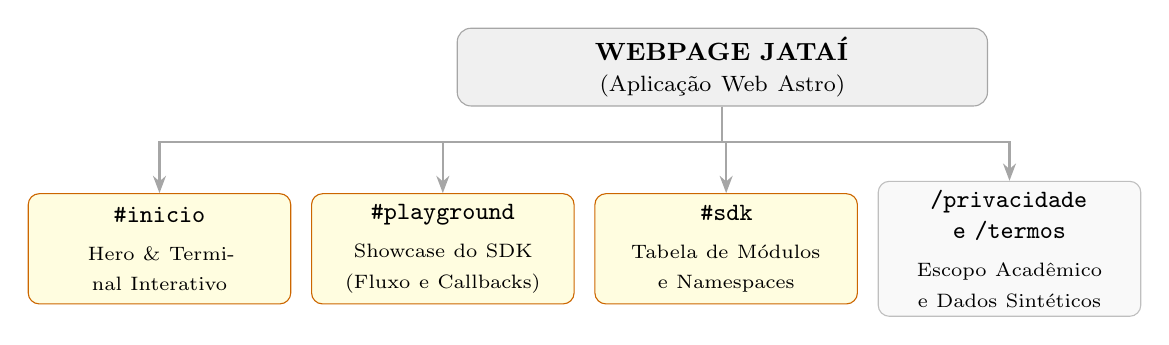
\begin{tikzpicture}[
    node distance=0.5cm and 0.25cm,
    auto,
    root/.style={rectangle, draw=gray!70, fill=gray!12, rounded corners=5pt, text width=6.5cm, align=center, font=\bfseries\small, minimum height=0.9cm},
    navnode/.style={rectangle, draw=orange!80!black, fill=yellow!12, rounded corners=4pt, text width=3.1cm, align=center, font=\small, minimum height=1.4cm},
    legalnode/.style={rectangle, draw=gray!50, fill=gray!5, rounded corners=4pt, text width=3.1cm, align=center, font=\small, minimum height=1.4cm},
    line/.style={draw, -{Stealth[length=2.2mm]}, thick, gray!70}
]

    \node [root] (root) {WEBPAGE JATAÍ\\{\footnotesize\normalfont (Aplicação Web Astro)}};

    \node [navnode, below left=1.1cm and 2.1cm of root] (hero) {
        \textbf{\texttt{\#inicio}}\\[0.1cm]
        {\scriptsize Hero \& Terminal Interativo}
    };

    \node [navnode, right=0.25cm of hero] (playground) {
        \textbf{\texttt{\#playground}}\\[0.1cm]
        {\scriptsize Showcase do SDK (Fluxo e Callbacks)}
    };

    \node [navnode, right=0.25cm of playground] (sdk) {
        \textbf{\texttt{\#sdk}}\\[0.1cm]
        {\scriptsize Tabela de Módulos e Namespaces}
    };

    \node [legalnode, right=0.25cm of sdk] (legal) {
        \textbf{\texttt{/privacidade e /termos}}\\[0.1cm]
        {\scriptsize Escopo Acadêmico e Dados Sintéticos}
    };

    \draw [line] (root.south) -- ++(0,-0.45cm) -| (hero.north);
    \draw [line] (root.south) -- ++(0,-0.45cm) -| (playground.north);
    \draw [line] (root.south) -- ++(0,-0.45cm) -| (sdk.north);
    \draw [line] (root.south) -- ++(0,-0.45cm) -| (legal.north);

\end{tikzpicture}
\caption{Mapa de arquitetura funcional e seções navegáveis da página web da Jataí.}
\label{fig:site_arquitetura}
\legend{Fonte: Elaborado pelos autores (2026).}
\end{figure}

\subsection{Funcionalidades principais}
Alinhado à implementação real da interface em código, o portal oferece as seguintes capacidades:

\begin{itemize}
    \item{Terminal de abertura na hero (HeroTerminal):} componente interativo na seção principal que simula a execução imediata de requisições de Open Finance para rápida compreensão da proposta;
    \item{Playground de integração (ProductShowcase):} módulo onde o desenvolvedor acompanha passo a passo a simulação do uso do SDK em tempo real, desde a importação do pacote até o disparo e recebimento de callbacks;
    \item{Documentação modular da API (SdkModules):} tabela descritiva que organiza os namespaces do SDK em dois pilares principais:
    \begin{itemize}
        \item{Fluxo principal:} módulos de consentimento (\texttt{jatai.auth}), consulta de contas/saldos (\texttt{jatai.accounts}) e simulação de Pix (\texttt{jatai.payments});
        \item{Ferramentas do sandbox:} módulos para geração de cenários sintéticos (\texttt{jatai.data}) e injeção de latência/falhas (\texttt{jatai.telemetry}).
    \end{itemize}
    \item{Garantia de privacidade por dados sintéticos:} execução local e simulada, isenta de retenção de dados pessoais ou conexões bancárias reais, assegurando a conformidade acadêmica do projeto.
\end{itemize}

\chapter{Plano operacional}
\label{cap:plano_operacional}

O Plano Operacional descreve a dinâmica de funcionamento interno e externo da Jataí, detalhando o modelo de execução dos serviços, o fluxo estipulado para suporte e triagem de incidentes, os horários de operação, a infraestrutura física/remota e o ecossistema tecnológico empregado na sustentação da plataforma.

\section{Execução e prestação dos serviços}
\label{sec:execucao_servicos}

Os serviços são prestados sob a modalidade \textit{Software as a Service} (SaaS) e disponibilização de APIs (\textit{Application Programming Interfaces}). A entrega operacional ocorre em três frentes contínuas:

\begin{enumerate}
    \item{Provimento e disponibilização de ambientes (runtime):} manutenção das instâncias em nuvem dos simuladores (Jataí Core API, Pay Sandbox, Auth, Chaos \& Telemetry e DataGen), garantindo a disponibilidade das rotas e a execução dos dados sintéticos;
    \item{Distribuição de código e imagens de contêiner:} para os usuários do nível gratuito, a entrega é realizada via repositórios públicos no GitHub e imagens dockerizadas no Docker Hub, permitindo a execução local (self-hosted);
    \item{Gestão de chamados e atendimento técnico:} suporte contínuo para resolução de dúvidas comerciais, apoio na leitura de documentações e correção de eventuais falhas (bugs) identificadas nos sandboxes.
\end{enumerate}

\section{Atendimento e suporte técnico}
\label{sec:fluxo_atendimento}

Para assegurar a rastreabilidade e a rápida resolução de incidentes, o atendimento ao usuário é estruturado em dois níveis de suporte e alinhado aos princípios da notação BPMN (\textit{Business Process Model and Notation}). O fluxo completo de atendimento está ilustrado na Figura~\ref{fig:fluxo_atendimento}.

\begin{figure}[htbp]
    \centering
    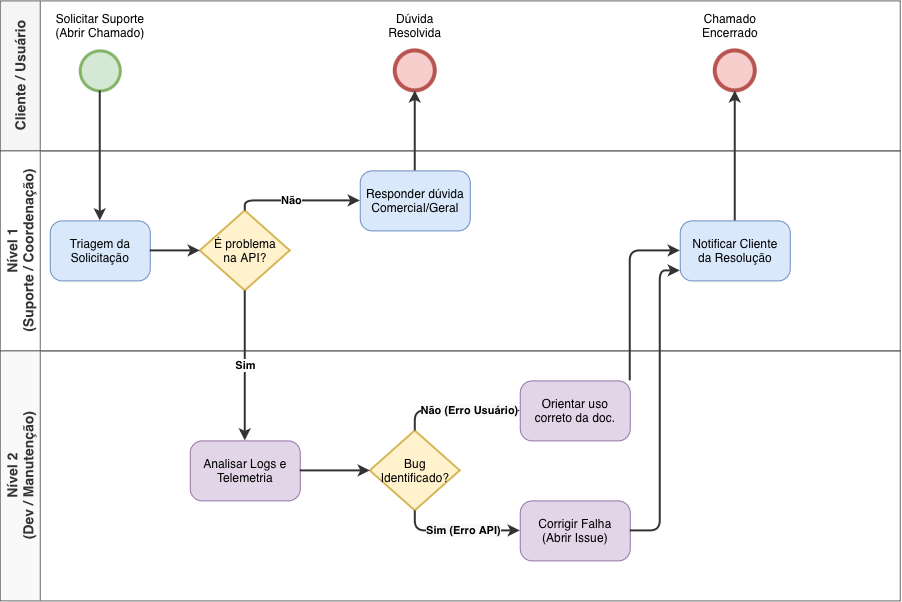
\includegraphics[width=0.98\textwidth]{fluxograma_atendimento.png}
    \caption{Fluxograma BPMN do processo de atendimento e suporte técnico.}
    \label{fig:fluxo_atendimento}
    \legend{Fonte: Elaborado pelos autores (2026).}
\end{figure}

\subsection{Detalhamento das etapas}
Como observado na Figura~\ref{fig:fluxo_atendimento}, a execução do suporte distribui-se:

\begin{itemize}
    \item{Cliente / usuário:} inicia o processo com a solicitação de suporte (abertura de chamado via formulário no portal ou portal de tickets). Acompanha a notificação de resolução até o encerramento do chamado;
    \item{Nível 1 — suporte e coordenação:} realiza a triagem inicial da solicitação.
    \begin{itemize}
        \item Caso o chamado trate de dúvidas comerciais ou gerais (não sendo um problema na API), o Nível 1 responde diretamente ao usuário, sanando a dúvida e encerrando o processo;
        \item Caso seja diagnosticado um problema na API, a solicitação é encaminhada imediatamente para análise técnica do Nível 2.
    \end{itemize}
    \item{Nível 2 — engenharia de desenvolvimento e manutenção:} recebe o chamado escalado e realiza a análise profunda de logs e dados de telemetria.
    \begin{itemize}
        \item Se não for um bug da API (erro do usuário/uso incorreto): o Nível 2 orienta sobre o uso correto da documentação e devolve a resolução ao Nível 1, que notifica o cliente e encerra o chamado;
        \item Se um bug for confirmado (erro na API): o Nível 2 efetua a correção da falha (abrindo a respectiva Issue no repositório do projeto), aciona o deploy de correção e devolve ao Nível 1 para notificar o cliente sobre a resolução.
        \item A retenção de logs de acesso segue as diretrizes do Marco Civil da Internet \cite{brasil2014marcocivil}.
    \end{itemize}
\end{itemize}

\section{Horários de funcionamento}
\label{sec:horario_funcionamento}

Dado o caráter digital da plataforma, os horários operacionais dividem-se em operação automatizada e atendimento humano.

\begin{itemize}
    \item{Disponibilidade dos ambientes de API (uptime):} operação automatizada 24/7 (vinte e quatro horas por dia, sete dias por semana) na nuvem, com janela de manutenção programada às sextas, entre 14h00 e 16h00;
    \item{Atendimento humano de suporte (níveis 1 e 2):} segunda a sexta-feira, das 14h00 às 16h00 (horário de Brasília);
    \item{Acordo de nível de serviço (Service Level Agreement - SLA):}
    \begin{itemize}
        \item{Plano Pro:} tempo máximo de primeira resposta em até 12 horas úteis;
        \item{Plano Advanced:} tempo máximo de primeira resposta em até 4 horas úteis e suporte prioritário na correção de bugs.
    \end{itemize}
\end{itemize}

\section{Infraestrutura operacional}
\label{sec:localizacao_infraestrutura}

A Jataí adota um modelo de operação remoto e descentralizado, dispensando a necessidade de uma sede física própria comercial. Esta abordagem reduz os custos fixos operacionais e está alinhada à cultura nativa digital de desenvolvimento de \textit{software}.

\begin{itemize}
    \item{Sede institucional e reuniões:} apoio institucional das instalações da Universidade (Laboratórios de Engenharia de Software e Computação), utilizado para reuniões formais de governança, assembleias e treinamentos presenciais;
    \item{Infraestrutura de hospedagem em nuvem:} os servidores operam em data centers da Amazon Web Services (AWS) localizados na região de São Paulo (\texttt{sa-east-1}), garantindo baixa latência para os clientes nacionais e alta conformidade com a LGPD.
\end{itemize}

\section{Equipamentos necessários}
\label{sec:equipamentos_necessarios}

Para a manutenção das operações, a equipe utiliza estações de trabalho individuais e infraestrutura em nuvem, conforme dimensionado na Tabela~\ref{tab:equipamentos_necessarios}.

\begin{table}[htbp]
\centering
\caption{Equipamentos necessários para operação.}
\label{tab:equipamentos_necessarios}
\resizebox{\textwidth}{!}{
\begin{tabular}{|l|c|p{7cm}|}
\hline
\textbf{Recurso / Equipamento} & \textbf{Qtd.} & \textbf{Finalidade Operacional} \\ \hline
Estações de Trabalho (Notebooks) & 3 & Desenvolvimento de código, simulações locais e gestão institucional (processadores $\ge 8$ núcleos, $16$GB RAM). \\ \hline
Conexão de Banda Larga Redundante & 3 & Acesso remoto aos ambientes de homologação, deploy e atendimento ao cliente. \\ \hline
Instâncias de Computação AWS EC2 & Variable & Processamento contínuo das rotas de API dos simuladores. \\ \hline
Banco de Dados Gerenciado AWS RDS & 1 & Armazenamento seguro de dados sintéticos e logs estruturados. \\ \hline
\end{tabular}
}
\legend{Fonte: Elaborado pelos autores (2026).}
\end{table}

\section{Stack tecnológica}
\label{sec:tecnologia_utilizada}

O ecossistema operacional é sustentado por um conjunto de tecnologias consagradas no mercado de desenvolvimento de \textit{software}, distribuídas por camadas funcionais na Tabela~\ref{tab:stack_tecnologica}.

\begin{table}[htbp]
\centering
\caption{Mapeamento da stack tecnológica da plataforma.}
\label{tab:stack_tecnologica}
\resizebox{\textwidth}{!}{
\begin{tabular}{|l|p{5.5cm}|p{6.5cm}|}
\hline
\textbf{Camada Operacional} & \textbf{Tecnologia / Ferramenta} & \textbf{Aplicação Prática} \\ \hline
\textbf{Desenvolvimento \& APIs} & Node.js / TypeScript, Java (Spring Boot) & Construção dos serviços RESTful e regras do \textit{Core API} e \textit{Pay Sandbox}. \\ \hline
\textbf{Segurança e Autenticação} & Keycloak / OpenID Connect & Sustentação do servidor de autenticação FAPI-1 no \textit{Jataí Auth}. \\ \hline
\textbf{Banco de Dados} & PostgreSQL, Redis & Persistência de dados sintéticos e armazenamento em memória para \textit{tokens} e cache. \\ \hline
\textbf{Infraestrutura \& DevOps} & Docker, Docker Compose, GitHub Actions & Conteinerização das aplicações e automação dos pipelines de integração contínua (CI/CD). \\ \hline
\textbf{Telemetria \& Caos} & OpenTelemetry, Grafana, Prometheus & Instrumentação de métricas de latência e injeção controlada de falhas. \\ \hline
\textbf{Atendimento \& Suporte} & GitHub Issues, Zendesk Free / Trello & Controle de chamados, rastreamento de bugs e gestão de prazos de atendimento. \\ \hline
\end{tabular}
}
\legend{Fonte: Elaborado pelos autores (2026).}
\end{table}

\chapter{Plano financeiro}
\label{cap:plano_financeiro}

O Plano Financeiro estabelece a viabilidade econômica e a sustentabilidade orçamentária. Em conformidade com a Lei nº 13.267/2016, a empresa opera sem fins lucrativos, revertendo integralmente seu superávit operacional para a manutenção da infraestrutura, capacitação dos membros e aprimoramento das soluções tecnológicas.

A modelagem financeira fundamenta-se nos princípios da \textit{Gestão Financeira Enxuta} (\textit{Lean Finance}), buscando minimizar o custo fixo inicial e manter o ponto de equilíbrio (Break-Even Point) em patamares reduzidos e de rápido alcance.

\section{Capital inicial e fontes de financiamento}
\label{sec:capital_inicial}

O capital inicial necessário para a estruturação e entrada em operação da Jataí foi estimado em R\$ 2.500,00. Este valor destina-se prioritariamente à legalização jurídica da empresa, contratação de serviços essenciais de infraestrutura e constituição de um fundo de reserva inicial. A Tabela~\ref{tab:capital_inicial} discrimina a alocação do investimento inicial.

\begin{table}[htbp]
\centering
\caption{Discriminação do capital inicial.}
\label{tab:capital_inicial}
\resizebox{\textwidth}{!}{
\begin{tabular}{|l|p{7.5cm}|c|}
\hline
\textbf{Categoria de Investimento} & \textbf{Descrição do Destino} & \textbf{Valor (R\$)} \\ \hline
Legalização e Cartório & Registro do Estatuto Social, ata da fundação e obtenção do CNPJ. & R\$ 800,00 \\ \hline
Infraestrutura de TI & Registro de domínio (\texttt{.dev}), certificados de segurança e reservas AWS. & R\$ 200,00 \\ \hline
Contas e Softwares & Licenciamento de ferramentas de gestão e serviços de e-mail corporativo. & R\$ 500,00 \\ \hline
Reserva de Contingência & Fundo de segurança operacional para cobrir oscilações de câmbio/nuvem. & R\$ 1.000,00 \\ \hline
\textbf{Total do Capital Inicial} & & \textbf{R\$ 2.500,00} \\ \hline
\end{tabular}
}
\legend{Fonte: Elaborado pelos autores (2026).}
\end{table}

\subsection{Origem dos recursos}
O aporte inicial será integralizado por meio de aporte próprio proporcional dos membros fundadores, complementado por eventuais editais de fomento à inovação acadêmica e apoio institucional da Universidade.

\section{Empréstimos e endividamento}
\label{sec:emprestimos}

A Jataí adota uma política rigorosa de alavancagem zero, estipulando a não contração de empréstimos bancários ou financiamentos com terceiros.

\subsection{Diretrizes de mitigação do risco financeiro}
\begin{itemize}
    \item{Vedação ao endividamento:} em consonância com as diretrizes do Movimento Empresa Júnior (MEJ), é proibida a captação de dívidas de curto ou longo prazo junto a instituições financeiras;
    \item{Cálculo de capacidade operacional:} toda expansão de servidor ou contratação de ferramentas deverá se subordinar à disponibilidade em caixa, garantindo que a operação nunca apresente saldo negativo;
    \item{Proteção orçamentária por trava de gastos (Hard Limits):} os serviços em nuvem (AWS) são configurados com alertas de faturamento automatizados e hard limits, interrompendo o provisionamento elástico antes de exceder o orçamento mensal previsto.
\end{itemize}

\section{Custos fixos}
\label{sec:custos_fixos}

Os custos fixos representam as despesas recorrentes e indispensáveis para manter a plataforma ativa e a empresa júnior juridicamente regularizada, independentemente do volume de requisições ou quantidade de assinantes. A Tabela~\ref{tab:custos_fixos} detalha a composição dos custos fixos mensais previstos.

\begin{table}[htbp]
\centering
\caption{Estrutura mensal de custos fixos.}
\label{tab:custos_fixos}
\resizebox{\textwidth}{!}{
\begin{tabular}{|l|p{7.5cm}|c|}
\hline
\textbf{Elemento de Custo} & \textbf{Descrição do Serviço} & \textbf{Custo Mensal (R\$)} \\ \hline
Infraestrutura Nuvem Base & Instância reservada de baixo custo AWS EC2/RDS para banco e APIs core. & R\$ 180,00 \\ \hline
Domínios e Comunicação & Manutenção do domínio principal, DNS gerenciado e e-mails institucionais. & R\$ 50,00 \\ \hline
Custos Administrativos & Taxas bancárias de conta PJ, contador de apoio e certidões jurídicas. & R\$ 50,00 \\ \hline
\textbf{Total de Custos Fixos Mensais} & & \textbf{R\$ 280,00} \\ \hline
\end{tabular}
}
\legend{Fonte: Elaborado pelos autores (2026).}
\end{table}

\section{Custos variáveis}
\label{sec:custos_variaveis}

Os custos variáveis estão diretamente correlacionados ao volume de requisições enviadas aos sandboxes e à quantidade de assinantes pagantes nos planos Pro e Advanced.

\begin{itemize}
    \item{Processamento e banda excedente (nuvem AWS):} estimado em R\$ 4,80 por usuário pagante/mês. Custo referente ao consumo proporcional de memória, IOPS de banco de dados e transferência de dados de saída (data egress);
    \item{Taxas de processamento de pagamento (gateway):} estimado em $5\%$ do valor de cada assinatura cobrada, referente à taxa de intermediação e emissão de cobranças automáticas via Pix/Cartão pelo gateway parceiro (ex: Asaas / Mercado Pago).
\end{itemize}

\section{Receitas e projeção de faturamento}
\label{sec:receita_estimada}

A receita da Jataí é derivada da comercialização das assinaturas recorrentes nos níveis Pro (R\$ 19,90/mês) e Advanced (R\$ 89,90/mês). O nível Gratuito atua como funil de atração (Freemium). Tabela~\ref{tab:projecao_receita} apresenta a evolução estimada da base de clientes e da receita bruta mensal para o primeiro ano de operação.

\begin{table}[htbp]
\centering
\caption{Projeção de base de clientes e receita bruta mensal (Ano 1).}
\label{tab:projecao_receita}
\resizebox{\textwidth}{!}{
\begin{tabular}{|l|c|c|c|c|}
\hline
\textbf{Fase Operacional} & \textbf{Assinantes Pro} & \textbf{Assinantes Adv.} & \textbf{Receita Pro (R\$)} & \textbf{Receita Adv. (R\$)} \\ \hline
\textbf{Fase 1: Piloto (M1-M3)} & 10 & 1 & R\$ 199,00 & R\$ 89,90 \\ \hline
\textbf{Fase 2: Expansão (M4-M6)} & 25 & 4 & R\$ 497,50 & R\$ 359,60 \\ \hline
\textbf{Fase 3: Maturidade (M7-M12)} & 60 & 10 & R\$ 1.194,00 & R\$ 899,00 \\ \hline
\end{tabular}
}
\legend{Fonte: Elaborado pelos autores (2026).}
\end{table}

Conforme projetado, a Receita Bruta Mensal atinge R\$ 288,90 na Fase 1, evolui para R\$ 857,10 na Fase 2 e consolida-se em R\$ 2.093,00 a partir do sétimo mês de operação.

\section{Demonstrativo do Resultado do Exercício (DRE Projetado)}
\label{sec:dre_projetado}

Para consolidar o fluxo orçamentário e demonstrar a sustentabilidade financeira, a Tabela~\ref{tab:dre_projetado} apresenta o DRE Projetado para a Fase de Maturidade (Mês 7 em diante).

\begin{table}[htbp]
\centering
\caption{Demonstrativo do Resultado do Exercício (DRE Mensal projetado - maturidade).}
\label{tab:dre_projetado}
\begin{tabular}{|l|c|}
\hline
\textbf{Rubrica Financeira} & \textbf{Valor Mensal (R\$)} \\ \hline
\textbf{(+) RECEITA BRUTA OPERACIONAL} & \textbf{R\$ 2.093,00} \\ \hline
(-) Taxas do Gateway de Pagamento ($5\%$) & (R\$ 104,65) \\ \hline
\textbf{(=) RECEITA LÍQUIDA OPERACIONAL} & \textbf{R\$ 1.988,35} \\ \hline
(-) Custos Variáveis de Nuvem (70 clientes $\times$ R\$ 4,80) & (R\$ 336,00) \\ \hline
\textbf{(=) MARGEM DE CONTRIBUIÇÃO TOTAL} & \textbf{R\$ 1.652,35} \\ \hline
(-) Custos Fixos Operacionais (Tabela~\ref{tab:custos_fixos}) & (R\$ 280,00) \\ \hline
\textbf{(=) SUPERÁVIT OPERACIONAL LÍQUIDO} & \textbf{R\$ 1.372,35} \\ \hline
\end{tabular}
\legend{Fonte: Elaborado pelos autores (2026).}
\end{table}

O superávit mensal gerado de R\$ 1.372,35 é integralmente direcionado ao fundo de reserva da empresa júnior, possibilitando o financiamento de bolsas de apoio acadêmico, participação em congressos e custeio de certificações técnicas para os colaboradores.

\section{Equilíbrio operacional (\textit{Break-Even Point})}
\label{sec:ponto_equilibrio}

O ponto de equilíbrio operacional indica a quantidade mínima de assinaturas pagantes necessárias para cobrir $100\%$ dos custos fixos e variáveis, resultando em saldo nulo. Considerando um ticket médio ponderado ($P$) de R\$ 29,90 por assinante e um custo variável médio unitário ($CV$) de R\$ 6,30 (incluindo processamento e taxa de gateway), a Margem de Contribuição Unitaria ($MC$) é obtida pela Equação~\ref{eq:margem_contribuição}:

\begin{equation}
\label{eq:margem_contribuição}
MC = P - CV = 29,90 - 6,30 = \mathrm{R\$}\ 23,60
\end{equation}

Aplicando a relação do ponto de equilíbrio em quantidade de assinantes ($Q_{PE}$), temos a Equação~\ref{eq:break_even}:

\begin{equation}
\label{eq:break_even}
Q_{PE} = \frac{\mathrm{Custos\ Fixos}}{MC} = \frac{280,00}{23,60} \approx 11,86\ \mathrm{assinantes}
\end{equation}

Portanto, a Jataí atinge seu ponto de equilíbrio operacional ao conquistar 12 assinantes pagantes (combinação entre planos Pro e Advanced). Esta meta é superada já na transição entre a Fase 1 e a Fase 2 do projeto, o que demonstra a baixa vulnerabilidade financeira e o elevado grau de exequibilidade do plano de negócios.

\chapter{Aspectos legais}
\label{cap:aspectos_legais}

A estruturação jurídica e regulatória foi desenhada para assegurar plena conformidade com o ordenamento jurídico brasileiro. Por atuar no desenvolvimento de softwares de simulação para o ecossistema financeiro, a empresa combina a regulação específica das empresas juniores com as diretrizes de proteção de dados e propriedade intelectual.

\section{Tipo jurídico}
\label{sec:tipo_juridico}

A Jataí constitui-se sob a forma jurídica de Associação Civil de Direito Privado, sem fins lucrativos, de caráter educacional e acadêmico, regulamentada formalmente pela Lei Federal nº 13.267, de 6 de abril de 2016 (Lei das Empresas Juniores).

\subsection{Características da natureza jurídica}
\begin{itemize}
    \item{Gestão autônoma e exercício acadêmico:} a empresa é gerida e executada exclusivamente por alunos matriculados em cursos de graduação da Instituição de Ensino Superior (IES), sob a orientação e supervisão de professores tutores;
    \item{Inexistência de lucro ou distribuição de dividendos:} todo o eventual superávit financeiro decorrente das assinaturas dos planos Pro e Advanced é revertido integralmente para a manutenção da infraestrutura tecnológica, capacitação dos membros e atingimento dos objetivos estatutários;
    \item{Regime de trabalho voluntário:} os integrantes não possuem vínculo empregatício com a empresa júnior, atuando sob o regime de trabalho voluntário, conforme regido pela Lei Federal nº 9.608/1998 (Lei do Voluntariado).
\end{itemize}

\section{Documentos necessários para abertura}
\label{sec:documentos_abertura}

A formalização perante os órgãos públicos e a IES exige a instrução de um conjunto documental específico. A Tabela~\ref{tab:documentos_abertura} detalha os documentos obrigatórios, suas finalidades e os órgãos de registro pertinentes.

\begin{table}[htbp]
\centering
\caption{Documentação exigida para abertura e regularização da Jataí.}
\label{tab:documentos_abertura}
\resizebox{\textwidth}{!}{
\begin{tabular}{|l|p{6.5cm}|p{5cm}|}
\hline
\textbf{Documento / Instrumento} & \textbf{Descrição e Conteúdo Principal} & \textbf{Órgão / Instância de Registro} \\ \hline
Estatuto Social & Define a missão, regras de governança, diretrizes de não lucratividade e estrutura diretiva. & Cartório de Registro Civil de Pessoas Jurídicas (RCPJ). \\ \hline
Ata de Fundação e Eleição & Registra a fundação da entidade e a posse da primeira Diretoria Executiva e Conselho. & Cartório de Registro Civil de Pessoas Jurídicas (RCPJ). \\ \hline
Inscrição no CNPJ & Cadastro Nacional da Pessoa Jurídica sob o código CNAE $94.99-5-00$ (Atividades associativas). & Receita Federal do Brasil (RFB). \\ \hline
Convênio / Acordo com a IES & Acordo de cooperação técnica e reconhecimento institucional da empresa júnior. & Reitoria / Direção do Centro Acadêmico da IES. \\ \hline
Termos de Trabalho Voluntário & Contratos individuais firmados com cada estudante participante (Lei nº 9.608/98). & Arquivo Interno de RH da Jataí. \\ \hline
\end{tabular}
}
\legend{Fonte: Elaborado pelos autores (2026).}
\end{table}

\section{Licenças e autorizações}
\label{sec:licencas_conformidade}

Dada a natureza das soluções oferecidas pela Jataí, o cumprimento das normas legais divide-se em quatro categorias:

\subsection{Isenção e enquadramento perante o Banco Central do Brasil (BACEN)}
A Jataí comercializa e disponibiliza ambientes de testes, simulação e dados sintéticos (sandboxes). 
\begin{itemize}
    \item A empresa não realiza liquidação financeira real, não custodia valores e não atua como Instituição Financeira (IF) ou Instituição de Pagamento (IP);
    \item Por se tratar do fornecimento de infraestrutura de software de teste, as atividades da Jataí dispensam autorização prévia de funcionamento junto ao Banco Central do Brasil, operando estritamente como provedora de tecnologia de simulação.
    \item O projeto foi desenhado segundo as diretrizes estabelecidas na Resolução Conjunta nº 1 \cite{bcb2020resolucao1}, garantindo a interoperabilidade do ecossistema.
\end{itemize}

\subsection{Conformidade com a Lei Geral de Proteção de Dados (LGPD - Lei nº 13.709/2018)}
A proteção da privacidade é um pilar arquitetural dos produtos da Jataí, atendendo aos princípios de Privacy by Design e Privacy by Default:
\begin{itemize}
    \item{Inexistência de dados pessoais reais:} o módulo Jataí DataGen utiliza algoritmos geradores para produzir dados puramente sintéticos e matematicamente anonimizados, imunes ao escopo de sanções da LGPD;
    \item{Tratamento de dados de clientes:} os dados cadastrais de usuários dos planos (nome, e-mail e CNPJ/CPF do contratante) são armazenados sob estrito consentimento e criptografia, exclusivamente para gestão de acesso e emissão de cobrança.
\end{itemize}

\subsection{Licenciamento de software e propriedade intelectual}
A proteção da propriedade intelectual do ecossistema é mantida sob modelo híbrido.
\begin{itemize}
    \item{Código open source (nível gratuito):} licenciado sob a licença MIT ou Apache 2.0, permitindo a livre inspeção, modificação e execução acadêmica;
    \item{Registro de marca no INPI:} depósito do registro da marca nomo-nominativa ``Jataí'' e do logotipo representativo no Instituto Nacional da Propriedade Industrial (INPI) sob a classe de serviços de software (Classe NCL 42).
\end{itemize}

\chapter{Sustentabilidade e responsabilidade social}
\label{cap:sustentabilidade_social}

A atuação da Jataí pauta-se pelo alinhamento aos critérios ESG (\textit{Environmental, Social, and Governance}), reconhecendo que o desenvolvimento de tecnologia para o setor financeiro deve ser acompanhado pelo compromisso ético, socioambiental e educacional. Como Associação Civil sem fins lucrativos gerida por estudantes universitários, a empresa reverte seu impacto operacional em benefício da comunidade acadêmica e do ecossistema de inovação aberta.

\section{Compromisso Ambiental}
\label{sec:acoes_ambientais}

Apesar de operar em um modelo totalmente digital e sem cadeia produtiva fabril física, a Jataí adota práticas ativas para mitigar a pegada de carbono da sua infraestrutura de software e conscientizar sobre a preservação ambiental.

\begin{itemize}
    \item{Computação verde na nuvem (Green Cloud Computing):} hospedagem dos contêineres e bancos de dados em provedor de nuvem (AWS - Região \texttt{sa-east-1}) comprometido com a transição para $100\%$ de energia renovável em seus data centers até 2025/2026. Além disso, a arquitetura do ecossistema utiliza rotinas de auto-desligamento (auto-scaling) para instâncias de teste inativas, evitando desperdício de processamento computacional;
    \item{Operação paperless (zero papel):} eliminação integral do uso de papel em processos internos, contratos e documentações. A gestão documental, emissão de certidões e disponibilização de manuais ocorrem exclusivamente em formato digital assinado eletronicamente;
    \item{Conscientização e preservação da biodiversidade:} inspirada pela abelha nativa Tetragonisca angustula (Jataí), a empresa destina parte de suas campanhas institucionais e portal web para a divulgação de ações de preservação de meliponídeos (abelhas sem ferrão) e da biodiversidade brasileira, em parceria com projetos de extensão universitária do meio ambiente.
\end{itemize}

\section{Democratização do conhecimento}
\label{sec:projetos_sociais}

A responsabilidade social da Jataí traduz-se no apoio direto à formação de novos talentos e na redução das barreiras de entrada para o ecossistema de Open Finance.

\begin{itemize}
    \item{Gratuidade e acesso livre ao código (tier gratuito):} disponibilização gratuita do código-fonte e das imagens de contêiner de todos os produtos (Jataí Core API, Pay Sandbox, Auth, Chaos e DataGen) para alunos de graduação, pós-graduação e pesquisadores de instituições públicas e privadas;
    \item{Programa "Jataí nas escolas e universidades":} oferta semestral de workshops e bootcamps gratuitos sobre arquitetura de APIs, segurança FAPI, LGPD e finanças digitais, direcionados a estudantes do ensino técnico e superior em situação de vulnerabilidade socioeconômica;
    \item{Incentivo à inovação aberta (open source):} estímulo à comunidade acadêmica para contribuição em repositórios públicos, permitindo que os alunos desenvolvam portfólio prático de engenharia de software antes de ingressarem no mercado de trabalho.
\end{itemize}

\section{Inclusão, acessibilidade e diversidade}
\label{sec:inclusao_acessibilidade}

\subsection{Diversidade e inclusão no quadro de membros}
Os processos seletivos semestrais da Jataí adotam ações afirmativas e mecanismos de equidade:
\begin{itemize}
    \item Processo seletivo cego nas etapas iniciais de avaliação técnica;
    \item Metas de representatividade de gênero, raça e estudantes ingressantes por cotas sociais na composição das diretorias e cargos de desenvolvimento;
    \item Flexibilidade de horários e modelo remoto para viabilizar a participação de alunos trabalhadores ou com responsabilidades familiares.
\end{itemize}

\section{Indicadores}
\label{sec:impacto_social}

O impacto gerado pela Jataí é mensurado continuamente por meio de indicadores quantitativos e qualitativos. A Tabela~\ref{tab:indicadores_esg} sintetiza as metas sociais e institucionais projetadas para os dois primeiros anos de operação.

\begin{table}[htbp]
\centering
\caption{Matriz de indicadores de impacto social e sustentabilidade.}
\label{tab:indicadores_esg}
\resizebox{\textwidth}{!}{
\begin{tabular}{|l|p{7cm}|c|}
\hline
\textbf{Eixo ESG} & \textbf{Indicador Mapeado} & \textbf{Meta (Ano 1 - Ano 2)} \\ \hline
\textbf{Social / Educação} & Estudantes e pesquisadores impactados pelo Plano Gratuito. & $> 250$ usuários \\ \hline
\textbf{Social / Capacitação} & Participantes em workshops e bootcamps gratuitos de APIs. & $> 100$ alunos \\ \hline
\textbf{Ambiental / Nuvem} & Redução de consumo ocioso via auto-desligamento de contêineres. & $30\%$ de economia de CPU \\ \hline
\textbf{Inclusão / Pessoas} & Percentual de membros de grupos sub-representados na equipe. & $\ge 40\%$ do quadro \\ \hline
\textbf{Governança} & Repositórios e documentações técnicas abertas e auditáveis. & $100\%$ Open Source \\ \hline
\end{tabular}
}
\legend{Fonte: Elaborado pelos autores (2026).}
\end{table}

A consolidação destas ações reforça o papel da Jataí não apenas como uma fornecedora de tecnologia de simulação, mas como um agente de transformação educacional, inclusão produtiva e inovação responsável no cenário do Open Finance brasileiro.

\chapter{Gestão da qualidade}
\label{cap:gestao_qualidade}

A nossa política de gestão da qualidade visa assegurar a confiabilidade técnica das APIs, a precisão das simulações financeiras e a satisfação contínua dos desenvolvedores e instituições parceiras. Por tratar-se de uma plataforma de infraestrutura tecnológica, a qualidade é mensurada tanto sob a ótica da experiência do usuário (Developer Experience, DX) quanto pelo rigor metrológico e operacional do software.

\section{Satisfação do cliente}
\label{sec:mensuracao_satisfacao}

A satisfação dos usuários dos planos Gratuito, Pro e Advanced é monitorada de forma automatizada e contínua por meio de três instrumentos complementares.

\begin{itemize}
    \item{Customer Satisfaction Score (CSAT) no suporte:} ao final de cada chamado encerrado pelo Nível 1 ou Nível 2 (conforme fluxo do Tópico 11), o usuário é convidado a responder a uma avaliação direta de 1 a 5 estrelas quanto à agilidade e clareza da solução apresentada;
    \item{Net Promoter Score (NPS) trimestral:} aplicação de pesquisa recorrente na webpage, mensurando a probabilidade de recomendação da suíte de sandboxes para outros desenvolvedores ($0$ a $10$);
    \item{Métricas de experiência do desenvolvedor:} coleta de métricas indiretas de uso, tais como o tempo médio para realizar a primeira chamada com sucesso (Time to First Hello World - TTFHW) e a taxa de assertividade da documentação OpenAPI.
\end{itemize}

\section{Indicadores de qualidade (KPIs e SLAs)}
\label{sec:indicadores_qualidade}

A garantia da qualidade operacional baseia-se em indicadores quantitativos monitorados em tempo real pela suíte \textit{Jataí Chaos \& Telemetry} e pelas ferramentas de gestão de chamados. A Tabela~\ref{tab:indicadores_qualidade} consolida os principais KPIs e suas respectivas metas de serviço.

\begin{table}[htbp]
\centering
\caption{Indicadores de qualidade (KPIs) da plataforma.}
\label{tab:indicadores_qualidade}
\resizebox{\textwidth}{!}{
\begin{tabular}{|l|p{6cm}|c|c|}
\hline
\textbf{Indicador / KPI} & \textbf{Descrição do Parâmetro} & \textbf{Meta Ótima} & \textbf{Frequência} \\ \hline
\textbf{Uptime das APIs} & Percentual de tempo em que os simuladores estão operacionais. & $\ge 99,5\%$ & Contínua (24/7) \\ \hline
\textbf{Latência p95} & Tempo de resposta das requisições no $95^{\circ}$ percentil. & $< 200\mathrm{~ms}$ & Mensal \\ \hline
\textbf{Cobertura de Testes} & Percentual de linhas de código cobertas por testes automatizados. & $\ge 85\%$ & Por \textit{Deploy} \\ \hline
\textbf{Tempo de Primeira Resposta} & Tempo médio para o primeiro retorno humano no suporte (SLA). & $< 4\mathrm{~h\ úteis}$ & Mensal \\ \hline
\textbf{MTTR (\textit{Mean Time to Repair})} & Tempo médio decorrido para correção e deploy de \textit{bugs} na API. & $< 8\mathrm{~h}$ & Mensal \\ \hline
\textbf{CSAT do Suporte} & Média das avaliações de atendimento pós-chamado. & $\ge 4,5 / 5,0$ & Mensal \\ \hline
\end{tabular}
}
\legend{Fonte: Elaborado pelos autores (2026).}
\end{table}

\section{Melhoria contínua (Ciclo PDCA)}
\label{sec:melhoria_continua}

A melhoria contínua dos processos da Jataí é institucionalizada por meio do ciclo PDCA (\textit{Plan-Do-Check-Act}), integrado às rotinas ágeis da equipe sob a coordenação do nível tático.

\begin{figure}[htbp]
\centering
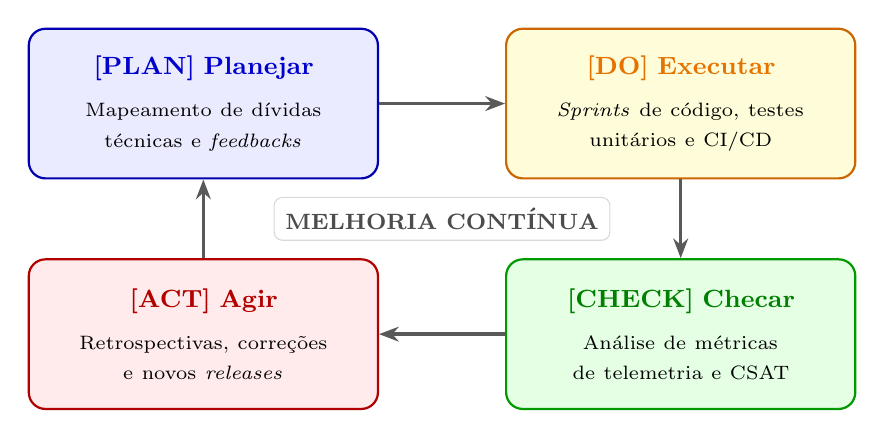
\begin{tikzpicture}[
    node distance=1.0cm and 1.6cm,
    auto,
    block/.style={
        rectangle, 
        draw, 
        rounded corners=6pt, 
        text width=4.2cm, 
        minimum height=1.9cm, 
        align=center, 
        font=\small,
        thick
    },
    line/.style={
        draw, 
        -{Stealth[length=2.5mm]}, 
        very thick, 
        gray!70!black
    }
]

    \node [block, fill=blue!8, draw=blue!70!black] (plan) {
        \textbf{\textcolor{blue!80!black}{[PLAN] Planejar}}\\[0.15cm]
        {\scriptsize Mapeamento de dívidas técnicas e \textit{feedbacks}}
    };

    \node [block, fill=yellow!15, draw=orange!80!black, right=of plan] (do) {
        \textbf{\textcolor{orange!90!black}{[DO] Executar}}\\[0.15cm]
        {\scriptsize \textit{Sprints} de código, testes unitários e CI/CD}
    };

    \node [block, fill=green!10, draw=green!60!black, below=of do] (check) {
        \textbf{\textcolor{green!50!black}{[CHECK] Checar}}\\[0.15cm]
        {\scriptsize Análise de métricas de telemetria e CSAT}
    };

    \node [block, fill=red!8, draw=red!70!black, below=of plan] (act) {
        \textbf{\textcolor{red!70!black}{[ACT] Agir}}\\[0.15cm]
        {\scriptsize Retrospectivas, correções e novos \textit{releases}}
    };

    \draw [line] (plan.east) -- (do.west);
    \draw [line] (do.south) -- (check.north);
    \draw [line] (check.west) -- (act.east);
    \draw [line] (act.north) -- (plan.south);

    \node [font=\bfseries\footnotesize, color=gray!60!black, fill=white, inner sep=4pt, rounded corners=3pt, draw=gray!30] 
        at ([xshift=0.8cm, yshift=-0.5cm]plan.south east) {MELHORIA CONTÍNUA};

\end{tikzpicture}
\caption{Representação do ciclo PDCA.}
\label{fig:ciclo_pdca}
\legend{Fonte: Elaborado pelos autores (2026).}
\end{figure}

\subsection{Engrenagens de Aplicação do Ciclo}
\begin{enumerate}
    \item{Plan (planejar):} priorização do backlog durante as reuniões de planejamento de sprint, correlacionando as solicitações dos usuários às metas de estabilidade da infraestrutura;
    \item{Do (executar):} implementação do código com esteiras de integração contínua (CI/CD via GitHub Actions) que bloqueiam pull requests que não atinjam os critérios mínimos de qualidade e cobertura de testes;
    \item{Check (checar):} auditoria mensal dos dashboards de telemetria, análise dos relatórios de estresse e compilação dos índices de satisfação dos usuários;
    \item{Act (agir):} realização de reuniões de retrospectiva de sprint para refinamento dos processos operacionais e atualização dos manuais técnicos da empresa.
\end{enumerate}

\section{Gestão de Incidentes}
\label{sec:tratamento_reclamacoes}

O tratamento de reclamações e falhas operacionais adota um protocolo estrito para evitar a recorrência de problemas e garantir transparência perante a comunidade de usuários.

\subsection{Fluxo de escalonamento}
Toda reclamação ou relato de insatisfação registrado nos canais formais recebe um nível de severidade:
\begin{itemize}
    \item{Severidade 1 (P1 - crítica):} indisponibilidade total de rotas core ou falha no servidor de autorização (Jataí Auth). Resposta imediata em até 1 hora e mobilização do Nível 2;
    \item{Severidade 2 (P2 - alta):} degradação de desempenho ou erro em endpoints secundários. Resposta em até 4 horas úteis;
    \item{Severidade 3 (P3 - moderada/baixa):} dúvidas na documentação, erros de digitação ou sugestões de melhoria. Resposta em até 12 horas úteis.
\end{itemize}

\subsection{Análise de Causa Raiz (\textit{Root Cause Analysis} - RCA) e Post-Mortem}
Para todo incidente classificado como Severidade 1 (P1), o Coordenador de Operações e QA conduz obrigatoriamente a técnica dos 5 Porquês para identificação da causa raiz. Ao final da resolução, é publicado um relatório de \textit{Post-Mortem} na webpage detalhando o impacto, a causa identificada, a solução aplicada e as ações preventivas adotadas para impedir que a falha se repita.

\chapter{Gestão de Riscos}
\label{cap:gestao_riscos}

Sob a supervisão direta da Coordenação de Operações, QA e Riscos (conforme governança do Capítulo~\ref{cap:estrutura_organizacional}), a empresa adota uma abordagem preventiva embasada no mapeamento de ameaças e na definição prévia de planos de contingência.

\section{Mapeamento dos riscos}
\label{sec:mapeamento_riscos}

As ameaças foram categorizadas em quatro dimensões fundamentais, considerando o modelo de negócios \textit{SaaS/Freemium} e a natureza acadêmico-empresarial de uma Empresa Júnior.

\subsection{Riscos financeiros}
\label{subsec:riscos_financeiros}
\begin{itemize}
    \item{Explosão de custos de nuvem (AWS Cost Overrun):} risco de consumo atípico de recursos computacionais ou banda excedente de dados (data egress) devido a picos não previstos de requisições ou ataques de negação de serviço, elevando a fatura da AWS acima do orçamento fixo;
    \item{Inadimplência ou cancelamento (Churn) de assinantes:} oscilação na receita recorrente mensal (MRR) proveniente dos planos Pro e Advanced, afetando a margem de contribuição necessária para cobrir os custos fixos da empresa;
    \item{Flutuação cambial (dólar vs. real):} como os serviços de nuvem têm precificação atrelada ao dólar americano (USD), variações cambiais bruscas podem impactar o custo operacional em moeda nacional (BRL).
\end{itemize}

\subsection{Riscos operacionais}
\label{subsec:riscos_operacionais}
\begin{itemize}
    \item{Rotatividade e perda de conhecimento (Turnover acadêmico):} risco inerente ao modelo de Empresa Júnior, caracterizado pelo desligamento natural de membros por conclusão de curso ou entrada no mercado de trabalho, podendo gerar Ponto Único de Falha (Single Point of Failure - SPOF) no conhecimento técnico;
    \item{Atraso no cronograma de entregas e suporte:} gargalos na capacidade operacional da equipe decorrentes de períodos de avaliações acadêmicas, resultando em estouro do SLA de atendimento de suporte;
    \item{Gargalo de homologação de código:} falhas na esteira de Quality Assurance (QA) que permitam a subida de código com falhas não detectadas para o ambiente de produção.
\end{itemize}

\subsection{Riscos de mercado}
\label{subsec:riscos_mercado}
\begin{itemize}
    \item{Baixa taxa de conversão para os planos pagos:} risco de adesão concentrada exclusivamente no plano gratuito (Self-hosted), com resistência dos desenvolvedores em migrar para os planos Pro ou Advanced;
    \item{Alterações regulatórias no Open Finance Brasil:} mudanças repentinas nas especificações de API e perfis de segurança (FAPI) emitidas pelo Banco Central do Brasil, exigindo refatorações estruturais urgentes nos simuladores;
    \item{Concorrência de ferramentas nativas ou institucionais:} lançamento de ambientes de sandbox gratuitos e oficiais por grandes instituições bancárias ou órgãos reguladores, reduzindo a atratividade comercial da plataforma.
\end{itemize}

\subsection{Riscos tecnológicos}
\label{subsec:riscos_tecnologicos}
\begin{itemize}
    \item{Vulnerabilidade de segurança no servidor de autenticação (Jataí Auth):} falhas na implementação dos protocolos OAuth 2.0 / FAPI que possam expor tokens de acesso ou permitir acessos não autorizados entre tenants;
    \item{Indisponibilidade da infraestrutura de nuvem (Outage AWS):} interrupção temporária dos serviços no data center do provedor em nuvem, afetando a disponibilidade garantida nos planos pagos;
    \item{Inconsistência algorítmica na geração de dados sintéticos (DataGen):} risco de geração de massas de dados incoerentes ou não relacionais que comprometam a qualidade dos testes executados pelos clientes.
\end{itemize}

\section{Matriz integrada de riscos}
\label{sec:matriz_riscos}

A Tabela~\ref{tab:matriz_riscos} consolida a matriz de riscos da Jataí, mensurando a probabilidade ($P$) e o impacto ($I$) de cada ameaça em uma escala ordinal de três níveis (\textbf{Baixo}, \textbf{Médio}, \textbf{Alto}) e estabelecendo as estratégias preventivas e corretivas de mitigação.

\begin{table}[htbp]
\centering
\caption{Matriz integrada de avaliação e mitigação de riscos.}
\label{tab:matriz_riscos}
\small
\resizebox{\textwidth}{!}{
\begin{tabular}{|p{3.2cm}|c|c|c|p{6.8cm}|}
\hline
\textbf{Risco Mapeado} & \textbf{Eixo} & \textbf{Prob.} & \textbf{Imp.} & \textbf{Estratégia de Mitigação e Contingência} \\ \hline

Explosão de Custos em Nuvem & Financ. & Média & Alto & Configuração de Hard Limits e Budget Alerts na AWS; limitação estrita de rate limit no API Gateway. \\ \hline

Rotatividade de Membros (SPOF) & Operac. & Alta & Alto & Documentação arquitetural rigorosa, pareamento de código (Pair Programming) e Programa Trainee contínuo. \\ \hline

Vulnerabilidade no Jataí Auth & Tecnol. & Baixa & Crit. & Testes automatizados de segurança (SAST/DAST), auditorias de código e alinhamento rígido às especificações FAPI-1. \\ \hline

Atrasos por Período Acadêmico & Operac. & Alta & Médio & Planejamento de sprints com folga orçada nos períodos de exames finais e escala de plantão no suporte. \\ \hline

Baixa Conversão de Planos & Mercado & Média & Médio & Fortalecimento da estratégia de DevRel, demonstrações interativas no site e oferta de trial do plano Pro. \\ \hline

Alteração Regulatória do BACEN & Mercado & Média & Alto & Monitoramento quinzenal das publicações do Open Finance e arquitetura de software modularizada. \\ \hline

Inconsistência no DataGen & Tecnol. & Baixa & Médio & Testes automatizados de validação de esquemas JSON e checagem de integridade referencial. \\ \hline

\end{tabular}
}
\legend{Fonte: Elaborado pelos autores (2026).}
\end{table}

\section{Planos de contingência}
\label{sec:planos_contingencia}

Para assegurar a rápida resposta diante da materialização dos riscos de maior impacto, a Jataí estabelece três protocolos específicos de contingência:

\subsection{Protocolo de trava orçamentária (Circuit Breaker Financeiro)}
Caso a fatura mensal projetada da AWS atinja $80\%$ do limite estipulado no orçamento fixo, o sistema aciona automaticamente a trava de consumo.
\begin{itemize}
    \item Desativação temporária da injeção de falhas complexas no módulo Jataí Chaos \& Telemetry;
    \item Aplicação de rate limiting mais severo nas instâncias públicas do nível Gratuito;
    \item Preservação integral do processamento e recursos dedicados aos usuários dos planos Pro e Advanced.
\end{itemize}

\subsection{Protocolo de transferência contínua de conhecimento}
Para eliminar o risco de dependência de membros específicos (SPOF):
\begin{itemize}
    \item Nenhuma funcionalidade é promovida para produção sem que o código tenha sido revisado e aprovado via Pull Request por pelo menos dois integrantes da equipe;
    \item Todo o conhecimento de infraestrutura, deploys e chaves de acesso é mantido de forma centralizada em cofres de senhas seguros (\textit{Vault}) e documentado no repositório interno da organização.
\end{itemize}

\subsection{Protocolo de recuperação de desastres (Disaster Recovery - DR)}
Em caso de indisponibilidade severa ou falha crítica de infraestrutura no provedor de nuvem:
\begin{itemize}
    \item Manutenção de rotinas automatizadas de backup diário do banco de dados relacional (AWS RDS);
    \item Infraestrutura como Código (IaC via scripts Docker/Terraform), permitindo a re-instanciação completa do ecossistema de APIs em uma nova região ou servidor em menos de 2 horas;
    \item Publicação imediata de comunicado e atualização nos meios de comunicação oficiais.
\end{itemize}

\chapter{Tecnologia e Inovação}
\label{cap:ferramentas_gestao_inovacoes}

Este capítulo consolida o suporte operacional, tecnológico e metodológico que viabiliza as atividades da Jataí. Apresenta-se o ecossistema de ferramentas adotado pela equipe, a metodologia de gestão ágil aplicada à governança e os vetores de inovação que posicionam a plataforma como solução pioneira de simulação para o Open Finance.

\section{Ferramentas utilizadas}
\label{sec:ferramentas_utilizadas}

Para garantir a eficiência operacional, o desenvolvimento contínuo e a comunicação fluida em um ambiente remoto, a Jataí selecionou uma suíte de ferramentas modernas, priorizando plataformas com integrações automatizadas e planos gratuitos para desenvolvedores ou entidades educacionais. A Tabela~\ref{tab:ferramentas_operacionais} categoriza as ferramentas adotadas de acordo com o domínio de aplicação.

\begin{table}[htbp]
\centering
\caption{Ferramentas utilizadas.}
\label{tab:ferramentas_operacionais}
\resizebox{\textwidth}{!}{
\begin{tabular}{|l|p{5.5cm}|p{6.5cm}|}
\hline
\textbf{Categoria / Domínio} & \textbf{Ferramentas Selecionadas} & \textbf{Finalidade Operacional} \\ \hline
\textbf{Gestão de Projetos \& Tarefas} & GitHub Projects / Trello & Organização do backlog, acompanhamento de sprints e quadros Kanban por diretoria. \\ \hline
\textbf{Comunicação \& Colaboração} & Discord / Google Workspace & Reuniões síncronas, alinhamentos diários (dailies), armazenamento em nuvem e e-mail institucional. \\ \hline
\textbf{Desenvolvimento \& Repositório} & GitHub, VS Code, Postman & Versionamento de código, revisão por pares (Pull Requests), testes de endpoints e documentação de APIs. \\ \hline
\textbf{Design \& Prototipação} & Figma, OpenAPI (Swagger UI) & Modelagem de interfaces do portal do desenvolvedor e renderização interativa de documentações técnicas. \\ \hline
\textbf{Infraestrutura \& CI/CD} & Docker, GitHub Actions, AWS Console & Conteinerização das APIs, automação de testes unitários/de carga e provisionamento de serviços em nuvem. \\ \hline
\textbf{Monitoramento \& Telemetria} & OpenTelemetry, Grafana, Prometheus & Monitoramento de métricas de desempenho (Uptime, latência e erros) do ambiente de produção. \\ \hline
\textbf{Gestão Financeira \& Jurídica} & Asaas / Mercado Pago, Cartório Digital & Emissão automatizada de cobranças por Pix/Cartão, emissão de NFS-e e assinatura eletrônica de termos. \\ \hline
\end{tabular}
}
\legend{Fonte: Elaborado pelos autores (2026).}
\end{table}

\section{Sistema de Gestão}
\label{sec:sistema_gestao}

A gestão da Jataí fundamenta-se no modelo Scrumban, uma abordagem híbrida que combina a previsibilidade do Scrum com a flexibilidade e o fluxo contínuo do Kanban. Esta escolha adapta-se perfeitamente à rotina universitária dos membros, permitindo entregas incrementais sem comprometer o desempenho acadêmico.

\subsection{Rituais e execução ágil}
\begin{itemize}
    \item{Sprints quinzenais (2 semanas):} ciclos de desenvolvimento e execução focados no cumprimento das metas priorizadas no backlog;
    \item{Reuniões de alinhamento (Standups síncronos e assíncronos):} três alinhamentos semanais curtos (15 minutos) via Discord ou checagens assíncronas no canal da equipe, identificando impedimentos e garantindo a cadência das entregas;
    \item{Sprint Planning e retrospectiva:} ao final de cada ciclo, a equipe realiza o planejamento do próximo período e a avaliação crítica dos processos internos, aplicando o ciclo PDCA para melhoria contínua (conforme detalhado no Capítulo~\ref{cap:gestao_qualidade}).
\end{itemize}

\subsection{Gestão por Objetivos e Resultados-Chave (OKRs)}
Para alinhar a visão estratégica das diretorias (Comercial, Operações, Marketing e Jurídico-Financeiro) às entregas semanais, a empresa adota a metodologia de OKRs (\textit{Objectives and Key Results}), com revisões trimestrais.

\section{Inovações propostas}
\label{sec:inovacoes_propostas}

A Jataí diferencia-se no mercado ao propor inovações disruptivas em três pilares fundamentais: tecnológico, de modelo de negócios e educacional.

\subsection{Inovação tecnológica}
Ao contrário dos sandboxes tradicionais que oferecem apenas respostas estáticas (mocked data), a Jataí introduz diferenciais técnicos inéditos no cenário de simulação do Open Finance:
\begin{itemize}
    \item{Geração estocástica de dados sintéticos (Jataí DataGen):} para garantir a conformidade com a LGPD \cite{brasil2018lgpd}, o Jataí DataGen gera massas de dados relacionais e cenários bancários completos imunes à LGPD, eliminando a necessidade de dados reais para testes de homologação;
    \item{Simulação de injeção de falhas (Jataí Chaos):} módulo que permite ao desenvolvedor simular cenários de alta latência, quedas de conexão, concorrência e erros de autorização FAPI, capacitando sistemas clientes a testarem sua resiliência antes da entrada em produção.
\end{itemize}

\subsection{Inovação no modelo de negócios}
\begin{itemize}
    \item{Abordagem freemium híbrida para Open Finance:} concessão de um nível totalmente gratuito (self-hosted via Docker) focado em desenvolvedores independentes e acadêmicos, eliminando a barreira financeira de entrada existente em soluções corporativas tradicionais;
    \item{Foco absoluto em experiência do desenvolvedor (DX):} documentação OpenAPI interativa e automatizada com princípio Time to First Hello World (TTFHW) inferior a 5 minutos, permitindo que qualquer equipe execute seu primeiro teste funcional rapidamente.
\end{itemize}

\subsection{Inovação social e educacional}
\begin{itemize}
    \item{Ponte de capacitação em arquitetura bancária avançada:} atuação da Empresa Júnior como ambiente de formação prática de alta complexidade (padrões FAPI-1, OpenID Connect, resiliência e telemetria), capacitando estudantes universitários em tecnologias de ponta demandadas pelo mercado financeiro global.
\end{itemize}

\chapter{Resultados esperados}
\label{cap:resultados_esperados}

A consolidação do ecossistema Jataí como plataforma de simulação para o \textit{Open Finance} visa gerar impactos mensuráveis de curto, médio e longo prazo. Os resultados esperados extrapolam o desempenho estritamente econômico-financeiro da empresa júnior, abrangendo a qualificação de capital humano, a redução de barreiras tecnológicas para o ecossistema de \textit{fintechs} e o fortalecimento do ensino prático de engenharia de \textit{software} no meio acadêmico.

\section{Número de pessoas e entidades atendidas}
\label{sec:pessoas_atendidas}

A estimativa do alcance da Jataí apoia-se em três eixos de público-alvo, sendo os desenvolvedores e empresas assinantes, comunidade acadêmica/estudantil e os membros integrantes da própria empresa júnior. A Tabela~\ref{tab:projecao_atendidos} apresenta a progressão quantitativa de impacto ao longo dos três primeiros anos de operação da plataforma.

\begin{table}[htbp]
\centering
\caption{Projeção trienal do número de pessoas e entidades impactadas.}
\label{tab:projecao_atendidos}
\begin{tabular}{|l|c|c|c|}
\hline
\textbf{Categoria de Público Atendido} & \textbf{Ano 1} & \textbf{Ano 2} & \textbf{Ano 3} \\ \hline
\textbf{Desenvolvedores / Startups (Pro e Advanced)} & 70 & 180 & 400 \\ \hline
\textbf{Estudantes e Pesquisadores (Tier Gratuito)} & 250 & 600 & 1.500 \\ \hline
\textbf{Participantes de Workshops e Bootcamps} & 100 & 250 & 500 \\ \hline
\textbf{Membros Formados pela EJ (Capacitação Interna)} & 15 & 35 & 60 \\ \hline
\textbf{Total Estimado de Impactados Diretos} & \textbf{435} & \textbf{1.065} & \textbf{2.460} \\ \hline
\end{tabular}
\legend{Fonte: Elaborado pelos autores (2026).}
\end{table}

\section{Impacto na comunidade}
\label{sec:impacto_comunidade}

O impacto social e comunitário da Jataí desdobra-se em três pilares fundamentais:

\subsection{Comunidade acadêmica e científica}
\begin{itemize}
    \item{Democratização do acesso a tecnologias bancárias:} eliminação da necessidade de orçamentos elevados ou contratos corporativos para que alunos e pesquisadores tenham acesso a cenários reais de simulação do Open Finance e padrões de segurança FAPI;
    \item{Fomento à pesquisa aplicada:} promoção do desenvolvimento de Trabalhos de Conclusão de Curso (TCC), dissertações e artigos científicos focados em engenharia de resiliência, sistemas distribuídos e geração estocástica de dados sintéticos.
\end{itemize}

\subsection{Ecossistema de tecnologia e startups}
\begin{itemize}
    \item{Aceleração do ciclo de inovação (Time-to-Market):} redução substancial do tempo gasto por fintechs e desenvolvedores independentes na criação manual de mocks e ambientes de testes;
    \item{Elevação da resiliência de softwares nacionais:} difusão da cultura de Chaos Engineering e testes de estresse antes do deploy em produção no mercado financeiro.
\end{itemize}

\subsection{Movimento Empresa Júnior (MEJ)}
\begin{itemize}
    \item{Posicionamento em Deep Tech:} estabelecimento de um modelo de referência para Empresas Juniores de tecnologia no Brasil, provando a viabilidade de desenvolver produtos de infraestrutura computacional de alto valor agregado no ambiente universitário.
\end{itemize}

\section{Crescimento Previsto}
\label{sec:crescimento_previsto}

A trajetória de crescimento da Jataí é pautada pela expansão gradual da base de usuários e pelo contínuo aprimoramento da arquitetura técnica.

\begin{itemize}
    \item{Escala de processamento de requisições:} salto estimado de 10 milhões de requisições simulação/mês no primeiro ano para mais de 100 milhões/mês até o terceiro ano, impulsionado pelo ganho de eficiência dos microsserviços;
    \item{Expansão do portfólio de simuladores:} evolução contínua da suíte de sandboxes para incorporar novos padrões regulatórios do Banco Central do Brasil, tais como Pix Automático, DREX (Real Digital) e interoperabilidade com Open Insurance;
    \item{Consolidação de parcerias estratégicas:} estabelecimento de acordos de cooperação com polos de inovação, incubadoras tecnológicas e hubs de fintechs.
\end{itemize}

\section{Benefícios econômicos e sociais}
\label{sec:beneficios_economicos_sociais}

A atuação da Jataí gera valor tangível tanto no âmbito financeiro-operacional dos seus clientes quanto no desenvolvimento social da comunidade universitária.

\subsection{Benefícios econômicos}
\begin{itemize}
    \item{Redução de custos de P\&D para clientes:} economia estimada de até $70\%$ nos custos de infraestrutura de homologação e testes para startups parceiras, que deixam de alocar engenheiros sêniores na criação de sandboxes proprietários;
    \item{Sustentabilidade financeira da EJ:} geração de superávit operacional constante para investimento no fundo de bolsas acadêmicas, custeio de certificações técnicas internacionais (AWS, Kubernetes, Java) para os membros da equipe e participação em congressos.
\end{itemize}

\subsection{Benefícios sociais}
\begin{itemize}
    \item{Inclusão produtiva e formação de talentos:} capacitação de estudantes do ensino público em ferramentas de ponta demandadas pelo mercado global de tecnologia, atuando como vetor de mobilidade social;
    \item{Proteção e conformidade com a LGPD:} promoção do uso ético de dados puramente sintéticos (Jataí DataGen), mitigando riscos de vazamento de dados sensíveis de cidadãos no ambiente de testes de software.
\end{itemize}

\chapter{Cronograma de criação}
\label{cap:cronograma_criacao}

O planejamento de elaboração e estruturação do Plano de Negócios da Jataí foi executado ao longo de três semanas, compreendendo o período de 03 de julho de 2026 a 24 de julho de 2026.

\section{Cronograma semanal de desenvolvimento}
\label{sec:cronograma_semanal}

O plano de trabalho foi fracionado em três etapas macro-operacionais, garantindo o encerramento rigoroso da documentação até a data limite estipulada de 24/07/2026.

\begin{itemize}
    \item{Semana 1 (03/07 a 09/07):}
    \begin{itemize}
        \item Definição do problema, proposta de valor e ecossistema de produtos (\textit{Jataí Core API}, \textit{Pay Sandbox}, \textit{Auth}, \textit{Chaos} e \textit{DataGen});
        \item Mapeamento do setor, análise de concorrência e público-alvo (Desenvolvedores, \textit{Fintechs} e Acadêmicos);
        \item Estruturação da matriz organizacional, governança da Empresa Júnior e matriz RACI.
    \end{itemize}
    
    \item{Semana 2 (10/07 a 16/07):}
    \begin{itemize}
        \item Definição do modelo de preços \textit{Freemium} (Gratuito, Pro R\$ 19,90 e Advanced R\$ 89,90);
        \item Desenho do fluxo de atendimento ao cliente em nota BPMN Bizagi (Suporte N1 e N2);
        \item Planejamento financeiro: projeção de custos fixos, variáveis, DRE e Ponto de Equilíbrio.
    \end{itemize}
    
    \item{Semana 3 (17/07 a 24/07):}
    \begin{itemize}
        \item Mapeamento do enquadramento legal (Lei nº 13.267/2016) e conformidade LGPD/BACEN;
        \item Definição das políticas ESG, Gestão da Qualidade (PDCA), Riscos e Contingências;
        \item Consolidação das ferramentas operacionais, inovações, resultados esperados e entrega final em 24/07/2026.
    \end{itemize}
\end{itemize}

\section{Cronograma bisual}
\label{sec:grafico_gantt}

A Figura~\ref{fig:grafico_gantt} ilustra o Gráfico de Gantt do projeto, mapeando o encadeamento temporal e a sobreposição das atividades ao longo das três semanas de execução.

\begin{figure}[htbp]
\centering
\resizebox{\textwidth}{!}{
\begin{ganttchart}[
    x unit=0.55cm,
    y unit title=0.6cm,
    y unit chart=0.65cm,
    vgrid,
    hgrid,
    title height=1,
    title label font=\bfseries\footnotesize,
    bar/.style={fill=blue!60, draw=blue!80},
    bar height=0.5,
    group right peaktip width=0.15
]{1}{21}
    % Cabeçalho de Datas (21 dias: 03/07 a 24/07)
    \gantttitle{Semana 1 (03-09/07)}{7}
    \gantttitle{Semana 2 (10-16/07)}{7}
    \gantttitle{Semana 3 (17-24/07)}{7} \\
    \gantttitlelist{3,4,5,6,7,8,9,10,11,12,13,14,15,16,17,18,19,20,21,22,23,24}{1} \\

    % Atividades
    \ganttgroup{1. Concepção \& Diagnóstico}{1}{7} \\
    \ganttbar{Visão do Produto \& Mercado}{1}{4} \\
    \ganttbar{Estrutura \& Governança EJ}{4}{7} \\
    
    \ganttgroup{2. Operação \& Finanças}{8}{14} \\
    \ganttbar{Estratégia Mkt \& Precificação}{8}{10} \\
    \ganttbar{Fluxo Operacional (BPMN)}{10}{12} \\
    \ganttbar{Plano Financeiro \& DRE}{12}{14} \\
    
    \ganttgroup{3. Legalidade \& Finalização}{15}{21} \\
    \ganttbar{Aspectos Legais \& ESG}{15}{17} \\
    \ganttbar{Qualidade \& Gestão de Riscos}{17}{19} \\
    \ganttbar{Consolidação \& Entrega Final}{19}{21} \\
    
    % Marco Final
    \ganttmilestone{Entrega (24/07)}{21}
\end{ganttchart}
}
\caption{Gráfico de Gantt.}
\label{fig:grafico_gantt}
\legend{Fonte: Elaborado pelos autores (2026).}
\end{figure}

\section{Resumo dos marcos do projeto (\textit{Milestones})}
\label{sec:marcos_projeto}

A Tabela~\ref{tab:marcos_projeto} resume os principais marcos do cronograma e suas respectivas datas de conclusão.

\begin{table}[htbp]
\centering
\caption{Marcos de Entrega do Plano de Negócios.}
\label{tab:marcos_projeto}
\resizebox{\textwidth}{!}{
\begin{tabular}{|l|p{8.5cm}|c|}
\hline
\textbf{Marco (\textit{Milestone})} & \textbf{Descrição do Entregável} & \textbf{Data de Conclusão} \\ \hline
\textbf{Escopo e Mercado} & Produto, análise setorial, público e estrutura jurídica da EJ. & 09/07/2026 \\ \hline
\textbf{Modelo de Negócio} & Precificação, fluxo BPMN e viabilidade financeira. & 16/07/2026 \\ \hline
\textbf{Governança e Risco} & LGPD, ações ESG, matriz de riscos e qualidade. & 21/07/2026 \\ \hline
\textbf{Versão Final} & Documento final revisado e formatado. & 24/07/2026 \\ \hline
\end{tabular}
}
\legend{Fonte: Elaborado pelos autores (2026).}
\end{table}

\postextual
\printbibliography[heading=bibintoc,title={Referências}]

\end{document}
